%%%%%%%%%%%%%%%%%%%%%%%%%%%%%%%%%%%%%%%%%%%%%%%%%%
%% Bachelor's & Master's Thesis Template        %%
%% Copyleft by Dawid Weiss & Marta Szachniuk    %%
%% Faculty of Computing and Telecommunication   %%
%% Poznan University of Technology, 2020        %%
%%%%%%%%%%%%%%%%%%%%%%%%%%%%%%%%%%%%%%%%%%%%%%%%%%


% Szkielet dla pracy licencjackiej pisanej w języku polskim.

\documentclass[polish,master,a4paper,oneside,11pt]{ppfcmthesis}


\usepackage[utf8]{inputenc}
\usepackage[OT4]{fontenc}
\usepackage{caption}
\usepackage{algorithm}
\usepackage{algpseudocode}
\usepackage{amsmath}
\usepackage{subfig}

\counterwithin{algorithm}{chapter}

%--------------------------------------
% Strona tytułowa
%--------------------------------------

% Autorzy pracy, jeśli jest ich więcej niż jeden
% wstaw między nimi separator \and
\author{%
   Bartosz Przybył \album{136785}}
\authortitle{}                                % Do not change.

\title{Poprawa klasyfikacji niezbalansowanych i zmiennych strumieni danych}

% Your supervisor comes here.
\ppsupervisor{prof.~dr hab.~inż.~Jerzy Stefanowski} 

% Year of final submission (not graduation!)
\ppyear{2022}                                 


\begin{document}

% Front matter starts here
\frontmatter\pagestyle{empty}%
\maketitle\cleardoublepage%

%--------------------------------------
% Podziękowania
\newpage\null\thispagestyle{empty}\newpage
\begin{center}
    \huge Podziękowania
\end{center}
Chciałbym złożyć podziękowania mojemu promotorowi, prof. dr hab. inż. Jerzemu Stefanowskiemu za inspirację tematem strumieni danych, cenne uwagi i wskazówki przekazywane od początku współpracy oraz poświęcony czas podczas tworzenia pracy.\\

\noindent Chciałbym także serdecznie podziękować dr hab. inż. Dariuszowi Brzezińskiemu prof. PP za wszelkie uwagi, wskazówki, poświęcony czas oraz inspirujące dyskusje, które nadały kształt tej pracy.

%--------------------------------------

% Streszczenie
\newpage\null\thispagestyle{empty}\newpage
\newpage
\begin{center}
    \huge Streszczenie
\end{center}
Nieustannie rosnąca liczba generowanych w dzisiejszym świecie danych sprawia, że tematyka eksploracji strumieni danych znacząco rozwinęła się w ostatnich latach. Dane strumieniowe mają coraz to większe rozmiary i bardziej złożoną charakterystykę, przez co wymagają coraz bardziej kompleksowych podejść, odpowiedzialnych za ich poprawną predykcję. Jednym z największych wyzwań, z którymi nie radzą sobie najlepiej aktualnie znane podejścia, jest klasyfikacja strumieni z określonymi typami zmian jak, np. dryf grup przykładów klasy mniejszościowej lub pojawianie się przykładów o różnym typie trudności. W ramach niniejszej pracy podjęto próbę stworzenia algorytmu, który byłby sobie w stanie poradzić z klasyfikacją takich strumieni. Efektem prac jest zaproponowanie trzech nowych podejść: \textit{Neighbourhood Undersampling Online Bagging (NUOB)}, \textit{Neighbourhood Oversampling Online Bagging} oraz \textit{Hybrid Neighbourhood Online Bagging (HNOB)}. W ramach oceny eksperymentalnej porównano zaproponowane podejścia wraz z dotychczas zaproponowanymi w literaturze. Przeprowadzone eksperymenty wykazały, że dla strumieni danych z przynajmniej dwoma czynnikami trudności zaproponowane klasyfikatory wykazują się wyższymi wartościami trafności predykcji ze względu na miary \textit{G-mean} oraz \textit{Recall}. Stan ten potwierdziły także testy statystyczne, które wskazały na statystyczną różnicę między nowymi a istniejącymi algorytmami.\\\\

\begin{center}
    \huge Abstract
\end{center}
The ever-increasing amount of data generated in today's world has caused the topic of data stream mining to develop significantly in recent years. Streaming data have increasingly large sizes and more complex characteristics, thus requiring more comprehensive approaches responsible for its correct prediction. One of the biggest challenges, which are not well-handled by currently known approaches, is the classification of data streams with specific changes like moving clusters of minority class examples or the appearance of examples of a particular type. This thesis attempts to create an algorithm that can cope with the classification of such streams. The work resulted in proposing three new approaches: \textit{Neighbourhood Undersampling Online Bagging (NUOB)}, \textit{Neighbourhood Oversampling Online Bagging} and \textit{Hybrid Neighbourhood Online Bagging (HNOB)}. The experimental evaluation compared the proposed approaches along with those proposed in the literature to date. The conducted experiments showed that for data streams with at least two difficulty factors, the proposed classifiers exhibit higher prediction accuracy values in terms of analyzing the metrics \textit{G-mean} and \textit{Recall}. Statistical tests also confirmed this condition, which indicated a statistical difference between the new and existing algorithms.

%--------------------------------------

%--------------------------------------
% Spis treści
%--------------------------------------
\newpage\null\thispagestyle{empty}\newpage
\newpage
\pagenumbering{Roman}\pagestyle{ppfcmthesis}%
\tableofcontents* 
\cleardoublepage % Zaczynamy od nieparzystej strony

%--------------------------------------
% Rozdziały
%--------------------------------------

%Najwygodniej jeśli każdy rozdział znajduje się w oddzielnym pliku
\mainmatter%
\chapter{Wstęp: Uczenie maszynowe w analizie strumieni danych}

\noindent W dzisiejszym świecie użytkownicy internetu przyzwyczajeni są do gromadzenia i udostępniania danych w dowolnym miejscu oraz o dowolnym czasie. Wraz ze wzrostem liczby ludzi posiadających dostęp do sieci oraz rozwojem technologii automatycznego gromadzenia i przechowywania informacji można zaobserwować wzrost rozmiarów przechowywanych danych. Zgromadzone zbiory mogą być szczególnie interesujące dla osób zajmujących się eksploracją danych, ze względu na możliwość odkrycia interesującej oraz wartościowej wiedzy reprezentowanej przez ukryte wzorce. Wyzwaniem w tym przypadku jest nie tylko efektywne przechowywanie danych, lecz także ich analiza, zdolność interpretacji i wyciągania użytecznych wniosków, które mogą prowadzić do lepszych decyzji \cite{DBrzezinski}\cite{Prezentacja:ZED}.

Według raportu \cite{Article:BigData} w samym roku 2021 na świecie wygenerowano około 79 zettabajtów danych. Szacunki na następne lata pokazują, że w roku 2022 może to być około 94 ZB, podczas gdy w 2025 roku liczba ta może osiągnąć nawet wartość ponad 150 ZB. Jednym z czynników wpływających na ogólną liczbę przetwarzanych informacji w dzisiejszym świecie są aplikacje, w których dane są generowane z bardzo dużą szybkością w postaci nieustannie zmieniających się \textit{strumieni danych}. Jako przykłady aplikacji generujących strumienie danych można wyszczególnić, np. systemy rekomendacyjne, systemy nawigacyjne w sztucznej inteligencji, systemy odpowiedzialne za badanie opinii w czasie rzeczywistym czy systemy odpowiedzialne za monitorowanie sieci komputerowych, telekomunikacyjnych i transakcji bankowych \cite{DBrzezinski:Prezentacja}.

Wspomniane wcześniej pojęcie \textit{strumienia danych} można opisać jako sekwencję elementów, które napływają w sposób ciągły w zmiennych interwałach czasu. Ze względu na ilość oraz szybkość napływania nowych przykładów eksploracja strumieni danych wymusza na badaczach uwzględnienie pewnych ograniczeń takich jak: ograniczony czas oraz ograniczona pamięć. Wspomniane ograniczenia sprawiają, że w środowisku strumieniowym nie jest możliwe przechowywanie w pamięci wszystkich przykładów, które napłynęły od początku działania danego algorytmu \cite{DBrzezinski}\cite{BrzezPhd2015}.

W standardowym ujęciu statycznego środowiska systemów uczących się, zbiór danych jest niezmienny oraz dostępny dla badacza przez cały czas. Przetwarzany zbiór danych może zostać poddany wielu modyfikacjom, każdy przykład ze zbioru może zostać przetworzony więcej niż jeden raz. Ze względu na wcześniej wspomniane ograniczenia: nieograniczoność zbioru danych (brak możliwości zapamiętania całego strumienia), krytyczny czas przetwarzania i odpowiedzi, jednorazowy odczyt elementu danych oraz możliwą zmienność rozkładów danych w czasie (\english{concept drift}) nie jest możliwe zastosowanie statycznych algorytmów eksploracji danych w środowisku strumieniowym \cite{Article:TradDataStream}\cite{Prezentacja:Strumienie}.

Zjawisko dryfu pojęć (\english{conecpt drift}), które można opisać jako zmiany definicji klas przewidywanych przez model w czasie, znacząco przyczyniło się do powstania nowych metod eksploracji strumieni, które radziłyby sobie ze zmiennością rozkładów danych. Do wspomnianych metod można zaliczyć okna przesuwne (\english{sliding windows}), detektory dryfu (\english{drift detectors}) czy modelowanie klasyfikatorów złożonych (\english{ensemble classifiers}) \cite{DBrzezinski}.

Ostatnimi czasy powstało wiele algorytmów podejmujących temat radzenia sobie ze zmiennością definicji klas przewidywanych przez model predykcyjny w czasie \cite{BrzezPhd2015}\cite{Article:ManyAlgorithms}\cite{Article:OBFirst}\cite{Article:OBSecond}. W pracach poświęconych konkretnym algorytmom do przetwarzania strumieni danych pokazano, że nowe metody przetwarzania są w stanie radzić sobie z niezbalansowanymi i zmiennymi strumieniami danych, ale tylko dla określonych scenariuszy. Wielu badaczy w swoich pracach jako zmianę w rozkładzie danych analizowali głównie zmianę globalnego współczynnika niezbalansowania między klasami (\english{imbalance ratio}). W artykule \cite{Article:TypyPrzykladow} zwrócono szczególną uwagę na dodatkowe czynniki, które poza zmianą liczności występowania przykładów z danych klas, wpływają na ogólną ocenę procesu klasyfikacji. Efektem końcowym pracy było zaprezentowanie tego, jak radzą sobie wybrane algorytmy w przypadku przetwarzania strumieni danych charakteryzujących się określonymi zmianami jak, np. podział klasy mniejszościowej na kilka mniejszych grup czy też napływ przykładów z klasy mniejszościowej określonego typu trudności. Szczególną uwagę zwrócono na analizę najbliższego sąsiedztwa danego przypadku, co pozwoliło na ostateczne określenie jego typu trudności jako przypadek bezpieczny, brzegowy, rzadki lub odstający (przyjęta konwencja została szerzej opisana w sekcji \ref{Section:DriftDataDistribution} niniejszej pracy). Wiele algorytmów radziło sobie bardzo dobrze na strumieniach charakteryzujących się występowaniem pojedynczego czynnika trudności w danych, jednak trafność predykcji znacząco spadała w przypadku, gdy czynników trudności w analizowanych danych było więcej.

Kierując się powyższymi motywacjami w niniejszej rozprawie podjęto próbę rozszerzenia istniejących algorytmów ukierunkowanych na przetwarzanie strumieni danych w taki sposób, aby stworzone algorytmy były w stanie poradzić sobie z klasyfikacją strumieni danych charakteryzujących się czynnikami trudności opisanymi w pracy \cite{Article:TypyPrzykladow}.
\chapter{Cel i zakres pracy}

\noindent Celem pracy jest zaprojektowanie nowych algorytmów, skupiających się na przetwarzaniu niezbalansowanych i zmiennych strumieni danych, dla których rozważane spektrum zmian, poza zmianą globalnego współczynnika niezbalansowania (\english{global imbalance ratio}) obejmowałoby dodatkowe czynniki trudności takie jak np. podział grupy przykładów z klasy mniejszościowej na kilka mniejszych grup czy napływ przypadków określonego typu. Wymienione czynniki trudności zostały szerzej opisane w pracy \cite{Article:TypyPrzykladow} oraz sekcji \ref{Section:DriftDataDistribution}. W tym celu stworzone algorytmy będą korzystać ze sztucznych, specjalnie wygenerowanych strumieni danych, które będą zawierały specjalne, określone własności. Sposób generowania określonych strumieni danych został szczegółowo opisany w rozdziale \ref{Chapter:Generator}. Ostatecznym rezultatem pracy będzie zaprezentowanie szczegółowych wyników oraz wykresów pokazujących jak prezentują się zaproponowane modyfikacje na tle ich algorytmów bazowych/podstawowych.\\

\noindent Struktura i budowa pracy jest następująca:

\begin{itemize}
    \item W rozdziale 3 przedstawiono przegląd badań oraz literatury na temat eksploracji niezbalansowanych i zmiennych strumieni danych, podstawowe pojęcia z tej dziedziny oraz opisy istniejących algorytmów przetwarzania strumieni potrzebne do zrozumienia dalszej części pracy
    \item W rozdziale 4 szczegółowo został opisany wykorzystany generator strumieni danych, na podstawie którego wyników dokonywano późniejszego etapu uczenia algorytmów
    \item W rozdziale 5 zawarto propozycje własnych modyfikacji algorytmów bazowych wraz z ich szczegółowym opisem oraz motywacją odpowiadającą za wprowadzenie określonej modyfikacji
    \item W rozdziale 6 przedstawione zostały wyniki eksperymentów z testowania zaproponowanych algorytmów uczenia maszynowego wraz z porównaniem ich do istniejących już w literaturze algorytmów
    \item W rozdziale 7 przedstawiono podsumowanie niniejszej rozprawy wraz z możliwymi dalszymi kierunkami rozwoju tematu
\end{itemize}

\newpage

\section{Wykorzystane narzędzia i technologie}

\begin{itemize}
    \item Języki programowania: \textit{Java}, \textit{Python}
    \item Biblioteki: \textit{Massive Online Analysis (MOA)}\cite{Article:MOA}, \textit{pandas}, \textit{numpy}, \textit{matplotlib}
    \item Środowiska programistyczne: \textit{IntelliJ IDEA Community Edition}, \textit{Microsoft Visual Studio Code}
\end{itemize}

\section{Środowisko eksperymentalne}

\noindent Wszystkie eksperymenty zostały wykonane na maszynie roboczej charakteryzującą się określonymi parametrami:

\begin{itemize}
    \item Procesor: Intel Core i5-6400 2.70 GHz
    \item Pamięć RAM: 8.00 GB
    \item Karta graficzna: NVIDIA GeForce GTX 970
    \item System operacyjny: Windows 10 Home
\end{itemize}
\chapter{Przegląd badań na temat niezbalansowanych i zmiennych strumieni danych}

\noindent W niniejszym rozdziale dokonano przeglądu badań oraz literatury na temat niezbalansowanych oraz zmiennych strumieni danych. Ponadto zostaną szczegółowo wytłumaczone pojęcia podstawowe konieczne do zrozumienia dalszej części pracy. Temat eksploracji strumieni danych rozwinął się znacząco w ostatnich latach. Na rynku jest widocznych coraz więcej nowych narzędzi skupiających się na przetwarzaniu strumieni danych. Do najbardziej znanych i popularnych możemy zaliczyć:

\begin{itemize}
    \item \textit{Massive Online Analysis (MOA)} - środowisko do implementowania oraz testowania algorytmów eksploracji strumieni danych, zawiera sporo algorytmów strumieniowych oraz pozwala na łatwe implementowanie nowych \cite{Article:MOA}
    \item \textit{River} - biblioteka służąca do przetwarzania strumieni danych w języku Python \cite{Article:River}
    \item \textit{SAMOA} - jest to rozproszona wersja środowiska MOA, zawiera nie tylko algorytmy, ale również łatwe API i narzędzia do testowania i porównywania algorytmów \cite{Article:Samoa}
    \item \textit{Apache Flink} - narzędzie umożliwiające eksplorację strumieni danych w wersji rozproszonej, określany jako ,,następca'' Sparka, posiada moduły do integracji np. z Kafką, Flume czy Twitterem \cite{Article:Flink}
\end{itemize}

\noindent Każde z zaprezentowane narzędzi posiada oddaną, swoją rzeszę użytkowników, którzy poprzez swój wkład wpływają na rozwój narzędzi do przetwarzania strumieni danych. Wraz z rozwojem narzędzi nie mogło także zabraknąć rozwoju pod kątem coraz to bardziej zaawansowanych implementacji algorytmów działających w środowisku strumieniowym. Stosując coraz to nowsze podejścia użytkownicy starają się o ciągłą poprawę swoich wyników klasyfikacji oraz o zniwelowanie wartości czynników, które negatywnie wpływały na wartość końcową klasyfikacji. 

Przegląd prac naukowych dotyczących klasyfikacji niezbalansowanych i zmiennych strumieni danych posłużył do wstępnej selekcji algorytmów przetwarzania strumieniowego, które można by było rozszerzyć w taki sposób, aby radziły sobie z dodatkowymi trudnościami opisanymi w pracy \cite{Article:TypyPrzykladow}.

Najczęściej przejawiającym się algorytmem w analizowanych artykułach naukowych był \textit{Online Bagging} oraz wszelkie jego odmiany i rozszerzenia \cite{Article:TypyPrzykladow}\cite{Article:ManyAlgorithms}\cite{Article:OBFirst}\cite{Article:OBSecond}, co ukierunkowało naturalny wybór przetestowania i próby rozszerzenia tego algorytmu w opisywanej pracy. Warto także wspomnieć, że modyfikacje tego algorytmu charakteryzowały się wysokimi wynikami predykcji w stosunku do innych algorytmów opisywanych w innych publikacjach. Wybrane algorytmy przetwarzania strumieniowego zostały szczegółowo opisane w sekcji \ref{Teoria:Algorytmy}.

W ramach poniższej analizy oraz w celu zdefiniowania poniższych pojęć założono, że strumień danych może zostać zdefiniowany jako sekwencja elementów $S = \{x_t, y_t\}^{T}_{t=1}$, gdzie $x_t \in X$, $y_t \in Y$, $X$ w tym przypadku oznacza przestrzeń wielowymiarową o liczbie wymiarów równej liczbie atrybutów opisującej dany przykład (\english{input space}). W analizie będziemy skupiać się głównie na klasyfikacji binarnej, z tego względu $Y$ możemy zdefiniować jako zbiór $\{0,1\}$ (\english{output space}). Każdy z przykładów $(x_t, y_t)$ ma także przypisaną wartość z łącznego rozkładu prawdopodobieństwa strumienia opisaną jako $p_t(x,y)$ w chwili $t$ \cite{Article:TypyPrzykladow}. Założono także, że etykieta danego przykładu jest dostępna w momencie pojawienia się danego elementu w strumieniu.

\section{Dane niezbalansowane}

\noindent Dobór odpowiedniego algorytmu uczenia maszynowego może być nie tylko podyktowany jego wykorzystaniem we wszelakich, wcześniej omawianych pracach naukowych, ale także posiadanymi danymi i ich strukturą. W tematyce uczenia maszynowego wyszczególniamy dwa rodzaje danych: dane zbalansowane oraz dane niezbalansowane \cite{Article:Inz}.

Dane zbalansowane w tematyce eksploracji strumieni danych charakteryzują się tym, że przez cały okres napływania przykładów liczność elementów dla każdej z klas jest podobna - można powiedzieć, że każda z klas w dowolnym momencie działania algorytmu jest równoliczna.

Z kolei dane niezbalansowane w tematyce eksploracji strumieni danych są natomiast przeciwieństwem pojęcia danych zbalansowanych. Oznacza to, że gdy w analizowanym problemie klasyfikacji występują różne częstości pojawiania się obiektów należących do różnych klas, to problem taki należy traktować jako problem niezbalansowany - liczności klas w takim przypadku nie są równoliczne \cite{Article:Inz}.

Istotą problemu powyższego niezbalansowania jest przesłanka, że zastosowanie klasycznych mechanizmów uczenia na niezrównoważonym zbiorze danych może prowadzić do faworyzowania przez wyuczony klasyfikator klasy dominującej kosztem klasy zdominowanej. Innymi słowy, typowe podejście może skutkować skonstruowaniem modelu równoważnemu klasyfikatorowi, który przydziela wszystkim obiektom klasę dominującą, niezależnie od wartości wektora cech. Ze względu na zdecydowanie wyższą częstość pojawiania się obiektów z klasy dominującej w stosunku do klasy zdominowanej metoda charakteryzująca się niskim błędem klasyfikacji może charakteryzować się niskim (bądź zerowym) stopniem wykrywalności obserwacji z klasy zdominowanej \cite{MZieba}.

\label{Label:ImbalanceData}
W analizowanych przykładach strumień danych będzie oznaczony jako niezbalansowany w sytuacji, gdy w dowolnym momencie czasu $t$ zachodzi warunek $p_t(0) \ll p_t(1)$ lub $p_t(1) \ll p_t(0)$, gdzie $p_t(x)$ oznacza prawdopodobieństwo wystąpienia danego przykładu z klasy $x$ w chwili $t$. Klasa, która zawiera mniej przykładów jest nazywana klasą mniejszościową, natomiast z drugiej strony klasa zawierająca więcej przykładów nazywana jest klasą większościową. Aby określić globalny współczynnik niezbalansowania w strumieniu danych zdecydowano się na wykorzystanie wzoru $|S_{min}|/|S| * 100\%$, gdzie $|S_{min}|$ oznacza zaobserwowaną liczbę przykładów z klasy mniejszościowej, a $|S|$ oznacza zaobserwowaną ogólnę liczbę przykładów z wszystkich klas.

W niniejszej rozprawie problem niezbalansowania danych także występuje, przez co istnieje konieczność rozważenia jak sobie z nim poradzić. W celu uzyskania pełniejszego obrazu, bardziej szczegółowe wyjaśnienie dotyczące tego, jak algorytmy przetwarzania strumieni danych radzą sobie z problemem niezbalansowania danych, zostanie zaprezentowane w sekcji \ref{Teoria:Algorytmy}.


\section{Dryf pojęć}

\noindent Poza danymi niezbalansowanymi drugą składową tematu pracy są tzw. zmienne strumienie danych. Jak wcześniej wspomniano, za zmiany w strumieniu danych odpowiedzialne jest zjawisko nazywane dryfem pojęć (\english{concept drift}), które możemy zdefiniować jako zmiany definicji klas przewidywanych przez model w czasie.

Formalnie możemy opisać, że zjawisko dryfu pojęć wystąpiło w analizowanym strumieniu danych, jeśli dla dwóch różnych punktów w czasie $t$ i $t + \triangle$ warunek $\exists x : p_t(x, y) \ne p_{t + \triangle}(x, y)$ jest spełniony \cite{Article:DriftGama}\cite{Article:DriftGama2}.

Aby lepiej przedstawić to zjawisko posłużono się poniższą ilustracją:

\begin{figure}[h] 
    \centering\includegraphics[width=14cm]{figures/concept_drift_example.JPG}
    \caption{Przykładowe zjawisko dryfu pojęć na przykładzie klasyfikacji binarnej \cite{DBrzezinski:Prezentacja}}
\end{figure}

\noindent Powyższy rysunek rozważa problem klasyfikacji binarnej. Na samym początku analizy strumienia można wyznaczyć granicę decyzyjną między klasami, która modelowana jest przez pionową linię przechodzącą przez środek. Wraz z upływem czasu można zauważyć jak wcześniej zamodelowana granica decyzyjna zmienia się. W środkowej części ilustracji można zauważyć, że nie jest to już pionowa linia, a linia która skierowana jest po ukosie. Na końcu analizy strumienia granica decyzyjna jeszcze uległa zmianie i zamodelowana została jako linia pozioma przechodząca przez środek. Przez zaprezentowanie tego przykładu można dostrzec jak zmieniały się definicje klas przewidywanych przez model w czasie.

\subsection{Rodzaje dryfu ze względu na zmianę prawdopodobieństwa}

\noindent Na podstawie informacji zawartych w poprzedniej sekcji wiadomo, że dryf pojęć odnosi się do zmian w prawdopodobieństwie predykcji danej klasy w dwóch różnych momentach w czasie. W pracy \cite{Article:Kelly} zaprezentowano podejścia według których zjawisko dryfu pojęć może zajść w analizowanym strumieniu. Podejścia te odnoszą się do:

\begin{itemize}
    \item Zmian w prawdopodobieństwach wystąpień klas (prawdopodobieństwo a priori) - $p(y)$
    \item Zmian w prawdopodobieństwach wystąpień danego przykładu - $p(x)$
    \item Zmian w rozkładzie przykładów - $p(x|y)$
    \item Zmian w prawdopodobieństwach warunkowych klas (prawdopodobieństwo a posteriori) - $p(y|x)$
\end{itemize}

\noindent Ze względu na przyczynę i skutek opisanych zmian wyróżnia się dwa rodzaje dryfu \cite{Article:DriftGama2}:

\begin{itemize}
    \item Dryf rzeczywisty (\english{real drift})
    \item Dryf wirtualny (\english{virtual drift})
\end{itemize}

\noindent Dryf rzeczywisty (\english{real drift}) można zdefiniować jako dryf odnoszący się do zmian w prawdopodobieństwach warunkowych klas $p(y|x)$. Co warte zaznaczenia, taka zmiana może wystąpić bez ingerencji w prawdopodobieństwa wystąpień klas $p(y)$ oraz w prawdopodobieństwa wystąpień danego przykładu $p(x)$. Takie rozróżnienie jest niezwykle istotne, ponieważ niektóre metody eksploracji strumieni danych próbują wykrywać zjawisko dryfu pojęć wykorzystując wyłącznie wartości atrybutów \cite{Article:RealDrift}. Obecność dryfu rzeczywistego w strumieniu danych wpływa na przesuwanie się granic decyzyjnych pomiędzy klasami w miarę upływu czasu związanego z analizą.

Dryf wirtualny (\english{virtual drift}) należy zdefiniować jako dryf odnoszący się do zmian w prawdopodobieństwach wystąpień klas $p(y)$ lub w prawdopodobieństwach wystąpień danego przykładu $p(x)$. Warty wyszczególnienia jest fakt, że ten rodzaj dryfu nie wpływa na prawdopodobieństwa warunkowe klas $p(y|x)$, które pozostają niezmienne przez cały okres klasyfikacji danych ze strumienia \cite{Article:VirtualDrift}. Obecność dryfu wirtualnego w strumieniu nie powoduje zjawiska przesuwania się granic decyzyjnych pomiędzy klasami w miarę upływu czasu.

\newpage

Aby lepiej przedstawić i zrozumieć różnicę między tymi dwoma rodzajami posłużono się poniższą ilustracją:

\begin{figure}[h] 
    \centering\includegraphics[width=14cm]{figures/types_of_drift.JPG}
    \caption{Rodzaje dryfu pojęć na przykładzie klasyfikacji binarnej \cite{Article:DriftGama2}}
\end{figure}

\noindent Powyższy rysunek rozważa problem klasyfikacji binarnej. Na samym początku analizy można wyznaczyć granicę decyzyjną między klasami, która modelowana jest przez pionową linię przechodzącą przez środek. Kolejne dwie ilustracje (środkowa i po prawej) modelują rozkład danych w sytuacji, gdy wystąpił odpowiednio dryf rzeczywisty oraz dryf wirtualny. W przypadku dryfu rzeczywistego należy zauważyć jak zmiana w prawdopodobieństwach warunkowych klas $p(y|x)$ wpływa na zmianę granicy decyzyjnej pomiędzy klasami. Końcowo granica decyzyjna zostaje zamodelowana nie przez pionową linię przechodzącą przez środek, ale przez linię skierowaną na ukos. W przypadku dryfu wirtualnego należy zwrócić uwagę przede wszystkim na fakt, że zmiana w prawdopodobieństwach wystąpień danego przykładu $p(x)$ nie wpływa na zmianę granicy decyzyjnej pomiędzy klasami. Granica została zamodelowana w identyczny sposób jak dla danych z początku analizy strumienia.

\subsection{Rodzaje dryfu ze względu na sposób zmiany}

\noindent Kolejnym niemniej ważnym aspektem opisującym dryf pojęć jest sposób zmiany. Zjawisko dryfu pojęć można scharakteryzować ze względu na np. trwałość, dotkliwość, przewidywalność czy częstotliwość zmian \cite{Article:DriftType}\cite{Article:DriftType2}. Jednak najbardziej analizowanym aspektem dryfów jest sposób, w jaki przejawiają się one w czasie \cite{Article:DriftGama}\cite{Article:DriftType3}.

\newpage

\begin{figure}[h] 
    \centering
    \includegraphics[width=14cm]{figures/types_of_drift2.JPG}
    \caption{Rodzaje typów zmian zachodzących w analizie strumieni danych \cite{Article:DriftType4}}\label{Figure:DriftTypes}
\end{figure}

\noindent Na rysunku \ref{Figure:DriftTypes} przedstawiono sześć podstawowych typów zmian, które mogą wystąpić w analizie poszczególnego strumienia danych w miarę upływu czasu. Pierwszy z wykresów (\textit{Sudden}) jest odwzorowaniem nagłej i nieodwracalnej zmiany, która wpływa na natychmiastową zmianę przypisania elementów do klas. Kolejne dwa wykresy (\textit{Incremental} oraz \textit{Gradual}) są przykładem zmiany, która zachodzi w wolniejszym tempie, aniżeli to było dla przypadku wykresu \textit{Sudden}. Dla zmiany \textit{Incremental} można zaobserwować stałe, wolne tempo zmiany, które też można określić jako ciąg drobnych zmian. Typ \textit{Gradual} natomiast odnosi się w tym przypadku do zmiany w rozkładzie prawdopodobieństw pojawiania się kolejnych przykładów. Kolejny typ oznaczony jako \textit{Recurring} odnosi się do tymczasowej, krótkotrwałej i nagłej zmiany. W miarę upływu czasu sytuacja wraca do stanu początkowego. Warta podkreślenia jest kwestia, że ten typ zmiany nie jest określony jako cykliczny i dla badacza nie jest to potwierdzone, kiedy taka zmiana nastąpi ponownie. Fakt ten stanowi główną różnicę w porównaniu do zjawiska sezonowości wykorzystywanej w statystyce \cite{PHD:Zliobaite}. Typ oznaczony jako \textit{Outlier} reprezentuje pojedynczy, rzadki przypadek zmiany w danych generowane przez źródło. Ostatni z typów oznaczony jako \textit{Noise} reprezentuje losowe, niewielkie zmiany, które tak naprawdę nie są związane ze żadną zmianą w danych generowane przez źródło. Warto zwrócić uwagę na kwestię, że w przetwarzaniu strumieniowym nie powinno reagować się na typy oznaczone jako \textit{Outlier} oraz \textit{Noise} z tego względu, że reprezentują losowe, nie wnoszące pozytywnego aspektu do analizy zmiany. Wspomniane typy przy analizie strumieni danych powinny zostać zignorowane \cite{DBrzezinski}\cite{Prezentacja:Strumienie}.

\subsection{Rodzaje dryfu ze względu na rozkład danych}
\label{Section:DriftDataDistribution}

\noindent Ostatnim aspektem, na który warto zwrócić uwagę przy przedstawianiu zjawiska dryfu pojęć, są zmiany szczególnie związane z rozkładem danych. Ostatnio dokonane badania naukowe zidentyfikowały kluczowe własności danych, które utrudniają proces uczenia się z danych niezbalansowanych.

Jedną z takich własności jest globalny współczynnik niezbalansowania (\english{global imbalance ratio}), zdefiniowany jako procent liczby przykładów należących do klasy mniejszościowej w stosunku do liczby wszystkich przykładów (sekcja \ref{Label:ImbalanceData}). Jednym z wniosków wyciągniętych na podstawie badań był fakt, że wysoka miara współczynnika niezbalansowania nie zawsze pogarszała wyniki klasyfikacji. Wniosek ten doprowadził badaczy do wyłonienia innych, kluczowych własności danych, nazywanych także \textit{czynnikami trudności danych} (\english{data difficulty factors}), które zostały zaklasyfikowane jako źródła pogorszenia trafności klasyfikatorów.

Skupiając się na literaturze skoncentrowanej na uczeniu z statycznych, niezbalansowanych danych, można wyszczególnić następujące czynniki trudności \cite{Book:DataDistribution}\cite{Article:DataDistribution}:

\begin{itemize}
    \item Dekompozycja klasy mniejszościowej na kilka mniejszych grup (\english{the decomposition of the minority class concept into several sub-concepts})
    \item Obecność małych, odizolowanych grup przykładów z klasy mniejszościowej zlokalizowanych w głębi grupy elementów klasy większościowej (\english{the presence of small, isolated groups of minority examples located deep inside the majority class region})
    \item Efekt silnego nakładania się przykładów z różnych klas (\english{the effect of strong overlapping between the classes})
\end{itemize}

\noindent Każdy z wymienionych czynników odgrywa swoją rolę także w przetwarzaniu strumieniowym. Warto także zwrócić uwagę na fakt, że wystąpienie kilku różnych czynników w strumieniu danych znacząco wpływa na trafność klasyfikacji, stąd istnieje konieczność opracowania algorytmów, które radziłyby sobie z wymienionymi trudnościami. Poza wspomnianymi czynnikami należy także skupić się na innych czynnikach, które nie są obecne w procesie uczenia z danych statycznych, a występują w procesie uczenia na strumieniu danych. Przykładem takich czynników występujących w przetwarzaniu strumieniowym są operacje związane ze zmianami położenia grup przykładów w przestrzeni atrybutów.\\\\
\textbf{Dekompozycja klasy mniejszościowej na kilka mniejszych grup}\\

\noindent Badania eksperymentalne z wykorzystaniem różnych, rzeczywistych zbiorów danych wykazały, że klasa mniejszościowa zwykle nie tworzy jednego, spójnego regionu w przestrzeni atrybutów, ale często jest rozproszona w mniejszych grupach rozsianych po całej przestrzeni \cite{Book:DataDistribution}\cite{Article:DataDistribution2}\cite{Inbook:DataDistribution}. Naukowcy rozpoczęli badania nad wpływem dekompozycji klas na wydajność popularnych klasyfikatorów na kilku syntetycznych zbiorach danych \cite{Article:DataDistribution}. W ich eksperymentach skupisko stworzone z elementów klasy mniejszościowej, początkowo otoczony przykładami klasy większościowej, było sukcesywnie dzielone na kilka mniejszych grup, które były oddzielone przez regiony klasy większościowej. Wyniki pokazały, że zwiększenie podziału klasy mniejszościowej miało większy wpływ na trafność klasyfikacji aniżeli zmiana globalnego współczynnika niezbalansowania, zwłaszcza w przypadku mniejszej liczby przykładów \cite{Article:TypyPrzykladow}.\\\\
\textbf{Obecność małych, odizolowanych grup przykładów z klasy mniejszościowej zlokalizowanych w głębi grupy elementów klasy większościowej}\\

\noindent Zwykle są to grupy par, trójek przykładów z klasy mniejszościowej zlokalizowane dość daleko od granic decyzyjnych swojej klasy. Przyjmując koncepcję opisaną w \cite{Article:DataDistribution3} grupy takie nazywa się rzadkimi przypadkami (\english{rare cases}) i ze względu na ich rzadkość różnią się one od większych skupisk opisanych w sekcji dotyczącej dekompozycji. Z racji faktu, że klasa mniejszościowa jest niedoreprezentowana, nie można tych elementów traktować jako szumu. Na co warto zwrócić uwagę to fakt, że badania \cite{Article:DataDistribution2} dowiodły, że rzadkie przykłady, jeśli zostaną odpowiednio potraktowane, np. poprzez przetwarzanie wstępne (\english{pre-processing}), mogą być wykorzystane do poprawy predykcji klasy mniejszościowej. Należy pamiętać, że również pojedyncze przykłady mniejszościowe mogą znajdować się wewnątrz klasy większościowej lub w regionie pustej przestrzeni odgrywając rolę wartości odstających (\english{outlier}). Poprawne rozpoznanie takich przypadków jest niezwykle trudne, a większość metod specjalistycznych traktuje takie wartości odstające jako szum, dlatego w dalszych eksperymentach nacisk zostanie położony na poprawne rozpoznawanie rzadkich przypadków \cite{Article:TypyPrzykladow}.\\\\
\textbf{Efekt silnego nakładania się przykładów z różnych klas}\\

\noindent Efekt silnego nakładania się przypadków związany jest z nakładaniem się regionów przykładów z klasy mniejszościowej i większościowej w przestrzeni atrybutów. Czynnik ten jest obecny w wielu rzeczywistych zbiorach danych, a szczegółowe badania eksperymentalne wykazały, że jego rola jest jeszcze bardziej znacząca w przypadku danych niezbalansowanych, a w szczególności w przypadku klasy mniejszościowej. Autorzy pracy \cite{Article:DataDistribution4} wykazali, że zwiększenie liczby nakładających się obszarów pogorszyło wydajność sześciu popularnych klasyfikatorów w znacznie większym stopniu niż zmiana współczynnika niezbalansowania. Ponadto zaobserwowali oni także większy wypływ lokalnego współczynnika niezbalansowania w regionie nakładania się przykładów z różnych klas \cite{Article:TypyPrzykladow}.

\begin{figure}[h] 
    \centering
    \includegraphics[width=15cm]{figures/data_examples.JPG}
    \caption{Prezentacja rozkładów danych klasy mniejszościowej z określonymi czynnikami trudności \cite{Article:TypyPrzykladow}}\label{Figure:TypesExample}
\end{figure}

\noindent Na rysunku \ref{Figure:TypesExample} można zaobserwować graficzne odwzorowanie wszystkich wymienionych czynników. Klasa mniejszościowa na rysunku oznaczona jest kolorem zielonym. Na ilustracji \textbf{(a)} nie mamy do czynienia z czynnikami trudności, klasa mniejszościowa jest logicznie odseparowana od klasy większościowej. Przypadek \textbf{(b)} ilustruje sytuację dekompozycji klas mniejszościowej na kilka mniejszych skupisk, rozmieszczonych w kilku miejscach w przestrzeni atrybutów. Przypadek \textbf{(c)} pokazuje sytuację efektu silnego nakładania się przykładów z różnych klas. W celu ułatwienia interpretacji region nakładania się został wyszczególniony poprzez zaznaczenie jego granic dwoma linia. Ostatni z rysunków \textbf{(d)} przedstawia sytuację istnienia rzadkich oraz odstających przypadków z klasy mniejszościowej zlokalizowanych w głębi grupy elementów klasy większościowej. Jak można zauważyć grupy te są zdecydowanie mniejsze aniżeli te oznaczone na ilustracji \textbf{(b)} i najczęściej liczą dwa, trzy elementy (przypadki rzadkie) lub pojedyncze elementy (przypadki odstające).\\\\
\textbf{Rodzaje przykładów z klasy mniejszościowej ze względu na ich lokalne sąsiedztwo}\\

\noindent Analiza wspomnianych czynników trudności danych prowadzi do wyróżnienia różnych typów przykładów klasy mniejszościowej na podstawie liczby znajdujących się w ich pobliżu przykładów klasy mniejszościowej oraz większościowej \cite{Article:DataDistribution3}. Jedno z podejść do rozróżniania typów przykładów z klasy mniejszościowej \cite{Article:DataDistribution3}\cite{Article:DataDistribution2} analizuje etykiety klas przykładów w ich lokalnym sąsiedztwie zdefiniowanym przez k-najbliższych sąsiadów. W tym podejściu przykład z danej klasy oznaczany jest jako:

\begin{itemize}
    \item Bezpieczny (\english{safe}) - jeśli większość jego sąsiadów należy do tej samej klasy
    \item Brzegowy (\english{borderline}) - jeśli liczba etykiet sąsiadów z obu klas jest podobna
    \item Odstający (\english{outlier}) - jeśli wszyscy jego sąsiedzi należą do przeciwnej klasy
    \item Rzadki (\english{rare}) - jeśli liczba jego sąsiadów znajduje się pomiędzy granicami poziomu przypadku odstającego i brzegowego
\end{itemize}

\noindent Zaletą przyjęcia takiej konwencji przykładów bezpiecznych, brzegowych, odstających i rzadkich jest kwestia, że w ten sposób możliwe jest określenie udziału każdego typu przykładów z klasy mniejszościowej w procesie klasyfikacji na rzeczywistych zbiorach danych \cite{Article:TypyPrzykladow}\cite{Article:DataDistribution3}\cite{Article:DataDistribution2}.\\\\
\textbf{Zmiana pozycji grup obiektów}\\

\noindent Ostatnim z czynników trudności, który zostanie zaprezentowany, jest czynnik związany ze zmianą pozycji grup przykładów w przestrzeni atrybutów w miarę upływu czasu. Warta podkreślenia jest kwestia, że czynnik ten nie ma prawa wystąpić w analizie statycznych zbiorów danych ze względu na ich stałą, niezmienną strukturę. W przypadku strumieni danych rozważa się środowisko dynamiczne, w którym może dochodzić do zmian definicji klas przewidywanych przez model w czasie. W dotychczasowych pracach związanych nad analizą skupień w strumieniach danych próbowano modelować i monitorować ewolucję (przejścia) skupisk w czasie \cite{Article:ClusterTransition}. Przejścia te możemy podzielić na zewnętrzne i wewnętrzne.

\begin{itemize}
    \item Przejścia zewnętrzne - mogą być skategoryzowane jako podział skupiska na wiele mniejszych skupisk, zniknięcie skupiska, pojawienie się lub wchłonięcie przez inny skupisko
    \item Przejścia wewnętrzne - dotyczą jednego określonego skupiska, który może się rozszerzyć lub skurczyć w miarę upływu czasu, zmiana może także dotyczyć przesunięcia się środka skupiska lub całkowitej zmiany jego rozmieszczenia w przestrzeni atrybutów
\end{itemize}

\noindent Poprawne zamodelowanie oraz śledzenie zmian skupisk w analizie strumieni danych wpływa pozytywnie na ogólną trafność klasyfikacji, dlatego ważnym elementem w procesie projektowania algorytmu jest skupienie się na opisanym czynniku.

\section{Sposoby przetwarzania strumieni danych}

\noindent W dzisiejszym ujęciu analizy strumieni danych wyszczególniamy dwa podejścia przetwarzania strumieni danych. Pierwsze podejście skupia się na pojedynczym przetwarzaniu przykład po przykładzie w określonych momentach w czasie i jest określane przetwarzaniem przyrostowym (\english{online processing}). Celem drugiego podejścia jest przetwarzanie elementów strumienia w partiach, blokach o równym rozmiarze. Podejście takie jest określane przetwarzaniem blokowym (\english{block processing}).

\subsection{Przetwarzanie przyrostowe}

\begin{figure}[h] 
    \centering
    \includegraphics[width=15cm]{figures/online_processing.JPG}
    \caption{Proces uczenia ze strumienia danych w przetwarzaniu przyrostowym \cite{BrzezPhd2015}}\label{Figure:OnlineProcessing}
\end{figure}

\noindent Na rysunku \ref{Figure:OnlineProcessing} przedstawiono proces uczenia ze strumienia danych w przetwarzaniu przyrostowym. Tak jak wspomniano wcześniej, w tym podejściu każdy pojedynczy przykład zostaje przetworzony przez algorytm w momencie pojawienia się w strumieniu. Podejście to skupia się na przetwarzaniu przykład po przykładzie. Warto także zwrócić uwagę na okoliczność, że w momencie pojawienia się przykładu, najpierw wykonywana jest faza testowania modelu, a dopiero później model zostaje uaktualniony o wiedzę o tym przykładzie (faza uczenia). Taka ewaluacja nazywana jest oceną \textit{Test-then-train} i zostanie szczegółowo przedstawiona w sekcji \ref{Secton:TestThenTrain}.

\newpage

\subsection{Przetwarzanie blokowe}

\begin{figure}[h] 
    \centering
    \includegraphics[width=15cm]{figures/block_processing.JPG}
    \caption{Proces uczenia ze strumienia danych w przetwarzaniu blokowym \cite{BrzezPhd2015}}\label{Figure:BlockProcessing}
\end{figure}

\noindent Na rysunku \ref{Figure:BlockProcessing} przedstawiono proces uczenia ze strumienia danych w przetwarzaniu blokowym. Tak jak wspomniano wcześniej, celem tego podejścia jest przetwarzanie elementów strumienia w partiach, blokach o równym rozmiarze. Po zgromadzeniu odpowiedniej liczby przykładów w bloku danych, partia taka, podobnie jak to było we wcześniejszym podejściu, poddana zostaje najpierw fazie testowania na aktualnym modelu, a dopiero później następuje faza uczenia, gdzie model zostaje rozszerzony o dodatkową wiedzę pochodzącą z aktualnie przetworzonego bloku danych.

\noindent Warto także zwrócić uwagę na okoliczność, że przetwarzanie przyrostowe może zostać potraktowane jako szczególny przypadek przetwarzania blokowego, w którym wielkość każdego bloku $|B_j| = 1$

\section{Sposoby oceny algorytmów strumieniowych}

\noindent Eksploracja strumieni danych wymaga zdefiniowania własnych, oddzielnych sposóbów oceny algorytmów aniżeli te, które są znane z uczenia tradycyjnego. W uczeniu statycznym głównym podejściem, które jest najczęściej stosowane to podział zbioru danych na zbiór treningowy, testowy oraz walidacyjny. Dodatkowym czynnikiem, który często jest wykorzystywany przy ocenie algorytmów w środowisku statycznym jest wykonanie oceny krzyżowej (\english{cross-validation}). W środowisku dynamicznym nie jest możliwy fizyczny podział zbioru danych na zbiór treningowy, testowy oraz walidacyjny ze względu na nieograniczoność przypadków, które mogą pojawić się w takim strumieniu. Ponadto, tak jak to zostało wcześniej przedstawione, nie możliwe jest przechowywanie wszystkich przypadków, które pojawiły się w strumieniu, przez cały okres działania algorytmu, ze względu na ograniczoną pamięć. Dodatkowo w środowisku strumieniowym nie jest możliwe odtworzenie operacji oceny krzyżowej, z tego względu, że operacja taka jest zbyt kosztowna obliczeniowo - ograniczenie dotyczące czasu przetwarzania. Ze względu na restrykcje, które nakłada środowisko strumieniowe, powstało wiele specjalizowanych sposobów oceny algorytmów strumieniowych, które mają za zadanie ułatwić sprawdzenie trafności klasyfikacji dokonywanej na elementach strumienia.

\newpage

\subsection{Holdout}

\begin{figure}[h] 
    \centering
    \includegraphics[width=15cm]{figures/holdout.JPG}
    \caption{Sposób oceny algorytmów strumieniowych - \textbf{Holdout} \cite{Prezentacja:Strumienie}}\label{Figure:Holdout}
\end{figure}

\noindent Pierwszym z zaprezentowanych sposobów oceny algorytmów strumieniowych jest podejście \textit{Holdout}, zaprezentowane na rysunku \ref{Figure:Holdout}. Podejście to stara się być odwzorowaniem podziału na zbiór treningowy i testowy, znanego z uczenia statycznego. W tym sposobie tworzony jest niezależny zbiór testowy, do którego trafiają wybrane przykłady ze strumienia danych. Na podstawie tak stworzonego zbioru testowego dokonywana jest ocena procesu klasyfikacji na badanym strumieniu danych. Proces ten jest cykliczny, kolejne sprawdzenia dokonywane są na tym samym zbiorze testowym co określoną liczbę przykładów, które pojawią się w strumieniu (np. co milion przykładów) \cite{PHD:Kirkby}. Ze względu na stałą reprezentację zbioru testowego, metoda ta nie powinna być wykorzystywana do oceny strumieni danych, gdzie występuje dryf pojęć. Możliwość zmian w strumieniu powoduje, że przykłady znajdujące się w zbiorze testowym mogą być przestarzałe i nie powinny być wykorzystywane do oceny klasyfikatora.

\subsection{Test-Then-Train}
\label{Secton:TestThenTrain}

\begin{figure}[h] 
    \centering
    \includegraphics[width=15cm]{figures/online_processing.JPG}
    \caption{Sposób oceny algorytmów strumieniowych - \textbf{Test-Then-Train} \cite{Prezentacja:Strumienie}}\label{Figure:TestThenTrain}
\end{figure}

\noindent Drugim z zaprezentowanych sposobów oceny algorytmów strumieniowych jest podejście \textit{Test-Then-Train}, zaprezentowane na rysunku \ref{Figure:TestThenTrain}. Tak jak opisywano wcześniej, przy szczegółowym przedstawieniu sposobu przetwarzania przyrostowego, podejście to charakteryzuje się wykonaniem procesu testowania modelu na nowym przykładzie i następnie późniejszą fazą uczenia modelu na podstawie danych z nowego przykładu. Warto podkreślić fakt, że technika ta nie wymaga dodatkowej pamięci koniecznej na przechowywanie przykładów zbioru testowego. Metoda ta może być w pełni wykorzystywana do każdego rodzaju strumieni danych \cite{PHD:Kirkby}.

\subsection{Block-Based Evaluation}

\begin{figure}[h] 
    \centering
    \includegraphics[width=15cm]{figures/block_processing.JPG}
    \caption{Sposób oceny algorytmów strumieniowych - \textbf{Block-Based Evaluation} \cite{Prezentacja:Strumienie}}\label{Figure:BlockBasedEvaluation}
\end{figure}

\noindent Trzecim z zaprezentowanych sposobów oceny algorytmów strumieniowych jest podejście \textit{Block-Based Evaluation}, zaprezentowane na rysunku \ref{Figure:BlockBasedEvaluation}. Podejście to charakteryzuje się tym, że łączy cechy dwóch wcześniej opisanych sposobów. Trafność klasyfikacji oceniania jest nie na pojedynczych przykładach, tylko na blokach danych, a schemat działania jest ten sam, co w przypadku sposobu \textit{Test-Then-Train}. W pierwszej kolejności wykonywana jest faza testowania modelu na nowym bloku danych, po czym następuje faza uczenia modelu o nową wiedzę zawartą w przykładach w bloku. Metoda ta także może być w pełni wykorzystywana do każdego rodzaju strumieni danych \cite{DBrzezinski}.

\subsection{Prequential}

\begin{figure}[h] 
    \centering
    \includegraphics[width=15cm]{figures/prequential.JPG}
    \caption{Sposób oceny algorytmów strumieniowych - \textbf{Prequential} \cite{Prezentacja:Strumienie}}\label{Figure:Prequential}
\end{figure}

\noindent Ostatnim z zaprezentowanych sposobów oceny algorytmów strumieniowych jest podejście \textit{Prequential}, zaprezentowane na rysunku \ref{Figure:Prequential}. Podejście to także stara się wykorzystać cechy wcześniej opisanych sposobów oraz dodatkowo wprowadza swoje własne modyfikacje. Jedną z takich modyfikacji jest widoczna na rysunku metoda uczenia z wykorzystaniem okna przesuwnego (\english{sliding window}). Okno przesuwne w ocenie strumieni danych zawiera określoną liczbę najświeższych przykładów, które pojawiły się w strumieniu. Po pojawieniu się w strumieniu nowego przykładu, następuje usunięcie z okna przykładu najstarszego i ponowna ewaluacja trafności klasyfikacji. Kolejnym elementem, które wprowadza to podejście, jest współczynnik związany z zapominaniem najstarszych przykładów w oknie (\english{fading factor}). Współczynnik ten sprawia, że przykładom starszym, znajdującym się w oknie, zostaje przypisana niższa waga, aniżeli przykładom, które do tego okna niedawno trafiły. W ten sposób większy nacisk jest położony na naukę z najświeższych danych \cite{Article:Evaluation}.

\section{Miary oceny algorytmów strumieniowych}

\noindent W niniejszej sekcji przedstawione zostaną miary oceny, którymi możemy się posłużyć przy ocenie klasyfikatorów działających na strumieniach danych. W odróżnieniu od zaprezentowanych w poprzedniej sekcji sposobów oceny, tak w przypadku miar ocen algorytmów strumieniowych istnieje możliwość posłużenia się popularnymi miarami, które wykorzystuje się przy uczeniu z danych statycznych. Aby lepiej przedstawić najbardziej znane miary oceny zaprezentowana została poniższa macierz pomyłek dla problemu klasyfikacji binarnej:

\begin{center}
\begin{table}[h]
\renewcommand{\arraystretch}{1.5}
\label{tab:macierz}
\begin{center}
\begin{tabular}{|c|c|c|c|}
   \cline{3-4} 
   \multicolumn{1}{c}{} & & \multicolumn{2}{c|}{Predicted} \\ \cline{3-4}
   \multicolumn{1}{c}{} & & Positive & Negative \\ \hline
   
   {Observed}
   & Positive & TP & FN \\ \cline{2-4}
   & Negative & FP & TN  \\ \cline{2-4} \hline
\end{tabular}
\caption{Macierz pomyłek dla problemu klasyfikacji binarnej}
\end{center}
\end{table}
\end{center}

\noindent Założono, że klasa oznaczona jako \textit{Positive} oznacza klasę mniejszościową, podczas gdy klasa oznaczona jako \textit{Negative} oznacza klasę większościową. Wartości \textit{TP (True Positive)} oraz \textit{TN (True Negative)} oznaczają przypadki, w których klasyfikator dokonał poprawnej predykcji odpowiednio dla przykładu z klasy mniejszościowej i większościowej. Wartości \textit{FN (False Negative)} oraz \textit{FP (False Positive)} oznaczają przypadki, w których klasyfikator zaklasyfikował niepoprawnie odpowiednio przykład z klasy mniejszościowej i większościowej. Wykorzystując wprowadzone wartości wyszczególniono poszczególne miary ocen dla algorytmów klasyfikacji \cite{Inbook:Metrics}:

$$\textrm{Accuracy = }\frac{TP + TN}{TP + TN + FP + FN}$$
$$\textrm{Precision = }\frac{TP}{TP + FP}$$
$$\textrm{Sensitivity (Recall) = }\frac{TP}{TP + FN}$$
$$\textrm{Specificity = }\frac{TN}{TN + FP}$$
$$\textrm{G-mean = }\sqrt{\frac{TP}{TP + FN} \cdot \frac{TN}{TN + FP}}$$\\

\noindent Powyżej zostały zaprezentowane najbardziej popularne miary, wykorzystywane przy ocenie klasyfikatorów w uczeniu z danych statycznych. Wszystkie te miary mogłyby zostać z powodzeniem wykorzystane przy ocenie algorytmów bazujących na strumieniach danych. Należałoby jednak zwrócić uwagę na kwestię, że w pracy rozważany jest problem poprawy klasyfikacji niezbalansowanych i zmiennych strumieni, wobec czego nie wszystkie miary zostaną rozważone w dalszej części rozprawy. Jedną z takich miar jest miara trafności (\english{accuracy}), która dla algorytmów, predykujących zawsze klasę większościową, działających na strumieniach danych, gdzie 99\% przypadków stanowią elementy z klasy większościowej, osiągnąć może maksymalną wartość 99\%. Doszłoby w takim przypadku do faworyzowania przez wyuczony klasyfikator klasy dominującej kosztem klasy zdominowanej.

Należy szczególnie uważać na wspomniane zjawisko dominowania przez klasyfikator jednej klasy wobec drugiej, dlatego w niniejszej pracy zwracana jest szczególna uwaga na miary:

\begin{itemize}
    \item Czułości (\english{sensitivity}), która przekazuje informację, jaki procent przypadków z klasy mniejszościowej został sklasyfikowany pozytywnie
    \item Swoistości (\english{specificity}), która przekazuje informację, jaki procent przypadków z klasy większościowej został sklasyfikowany poprawnie
    \item G-mean, która jest pierwiastkiem z iloczynu miar czułości i swoistości, co oznacza, że kładzie nacisk na poprawną klasyfikację przypadków z obu klas, przy czym reaguje silniej na zjawisko faworyzowania aniżeli miara dokładności
\end{itemize}

Wymienione powyżej miary są bardzo często nieodłącznym elementem prac naukowych związanych z analizą niezbalansowanych i zmiennych strumieni danych \cite{Article:TypyPrzykladow}\cite{Inbook:Metrics}\cite{Article:OBFirst}\cite{Article:OBSecond}, wobec czego wybór tych właśnie miar do analizy w niniejszej rozprawie był naturalny.

\section{Algorytmy przetwarzania strumieni danych}
\label{Teoria:Algorytmy}

\noindent Tematyka związana z eksploracją strumieni danych była i jest poruszana w wielu pracach naukowych. Wraz z upływem lat w środowisku osób zajmujących się strumieniami danych możemy zauważyć powstawanie coraz to innych, rozbudowanych podejść do projektowania algorytmów przetwarzania. Wprowadzone algorytmy i specjalne podejścia można podzielić na cztery główne kategorie:

\begin{itemize}
    \item Pojedyncze klasyfikatory (\english{single classifiers})
    \item Techniki bazujące na wykorzystaniu okna (\english{windowing techniques})
    \item Detektory dryfu (\english{drift detectors})
    \item Klasyfikatory złożone (\english{ensemble approaches})
\end{itemize}

\subsection{Pojedyncze klasyfikatory}

\noindent Pojedyncze klasyfikatory są szczególnie znane z eksploracji danych w środowiskach statycznych. Co warte podkreślenia klasyfikatory te mogą zostać dostosowane w taki sposób, aby radziły sobie ze zmieniającymi się strumieniami danych. Klasyfikatorom działającym na danych statycznych, mimo możliwości przetwarzania sekwencyjnego danych, brakuje mechanizmu adaptacyjnego w stosunku do eksploracji strumieni danych. Na szczęście klasyfikatory takie można zmodyfikować w łatwy sposób zmodyfikować, aby reagowały na zmiany w strumieniach \cite{BrzezPhd2015}. 

W ramach tej grupy możemy wyszczególnić pięć rodzajów algorytmów:

\begin{itemize}
    \item Sieci neuronowe (\english{Neural networks}) \cite{Article:NeuralNetworks}
    \item Naiwny klasyfikator Bayesa (\english{Naive Bayes}) \cite{Article:NaiveBayes}
    \item Klasyfikatory oparte na najbliższym sąsiedztwie (\english{Nearest neighbour classifiers}) \cite{Article:Neighbours}
    \item Klasyfikatory wykorzystujące reguły decyzyjne (\english{Rule learners}) \cite{Article:DecisionRules}
    \item Drzewa decyzyjne (\english{Decision trees})
\end{itemize}

\noindent W zakresie niniejszej rozprawy szczegółowo zostanie wyjaśniony algorytm drzewa Hoeffding'a (\english{Hoeffding tree}), który należy do ostatniej grupy algorytmów - drzew decyzyjnych.\\\\
\textbf{Drzewo Hoeffding'a}\\

\noindent Drzewo Hoeffding'a można zdefiniować jako algorytm drzewa decyzyjnego służący do klasyfikacji danych strumieniowych. W klasycznym algorytmie drzewa decyzyjnego nie ma problemu z określeniem najlepszego atrybutu podziału. W przetwarzaniu strumieniowym nie jest możliwe określenie najlepszego atrybutu podziału, ze względu na brak wszystkich danych i nieograniczone pojawianie się kolejnych przykładów. Główną ideą tego algorytmu jest hipoteza, że często mała próbka danych może wystarczyć do określenia najlepszego atrybutu podziału drzewa decyzyjnego. Drzewo Hoeffding'a zostało dostosowane do nauki na danych strumieniowych poprzez wprowadzenie granicy Hoeffding'a, którą możemy zdefiniować w następujący sposób \cite{BrzezPhd2015}:

\begin{equation}
    \epsilon = \sqrt{\frac{R^2ln(1/\delta)}{2n}}
\end{equation}

\noindent gdzie:

\begin{itemize}
    \item $R$ - zakres wartości estymowanej funkcji
    \item $\delta$ - dopuszczalny błąd estymacji
    \item $n$ - rozmiar próbki
\end{itemize}

\noindent Drzewo Hoeffding'a działa w następujących etapach: 

\begin{enumerate}
    \item Zebranie odpowiednich statystyk z próbki strumienia
    \item Estymacja wartości funkcji oceny podziału dla każdego atrybutu
    \item Wykorzystanie granicy Hoeffding'a do zagwarantowania wyboru atrybutu podziału
\end{enumerate}

\newpage

\begin{figure}[h] 
    \centering
    \includegraphics[width=15cm]{figures/hoeffding_tree.JPG}
    \caption{Przykład budowy drzewa Hoeffding'a \cite{Prezentacja:Strumienie}}\label{Figure:HoeffdingTree}
\end{figure}

\noindent Na podstawie rysunku \ref{Figure:HoeffdingTree} można zaobserwować przykładowy proces wyboru atrybutu podziału w drzewie Hoeffding'a. Po wykonaniu drugiego etapu (estymacji wartości funkcji oceny dla każdego atrybutu) algorytm jest w stanie wybrać dwie największe wartości funkcji oceny i sprawdzić czy różnica między nimi jest większa niż oszacowana wartość granicy Hoeffding'a. Jeśli różnica ta jest większa to tworzony jest w drzewie nowy warunek podziału, w przeciwnym razie drzewo pozostaje w niezmienionej formie. Warto też zwrócić uwagę na fakt, że granica Hoeffding'a jest prawdziwa dla dowolnego rozkładu danych, co oznacza, że badacz podczas eksploracji nie musi martwić się o to, żeby jego dane pochodziły np. z rozkładu normalnego czy dwumianowego.

Pojęcie granicy Hoeffding'a było ważnym aspektem w kontekście analizy strumieni danych i przyczyniło się do powstania jednego z bardzo znanych algorytmów w analizie strumieni danych - Very Fast Decision Tree (VFDT) \cite{Article:VFDT}. Analizując ten algorytm warto także zwrócić uwagę na pracę \cite{Article:Rutkowski}, która wykazała, że w pierwotnej propozycji algorytmu źle zastosowano zastosowano granicę Hoeffding'a. W tej samej pracy autorzy pokazali także, że ograniczenie Hoeffding'a może zostać zastąpione innymi rozwiązaniami pochodzącymi z probabilistyki, np. nierównością McDiarmida (\english{McDiarmid's inequality}) \cite{Article:Rutkowski}.

\subsection{Techniki bazujące na wykorzystaniu okna}

\noindent Wiele algorytmów do analizy strumieni danych wykorzystuje techniki opierające się na użyciu okna. Najczęściej pojawiającą się formą okna w literaturze są okna przesuwne (\english{sliding windows}). Zadaniem okna przesuwnego jest ograniczenie liczby przykładów, które biorą udział w procesie uczenia. Ponadto okno przesuwne dba o to, żeby były to zawsze najświeższe przykłady. Najstarsze przykłady są usuwane z okna po pojawieniu się nowych przykładów. Ważną własnością okien przesuwnych jest fakt, że za ich pomocą istnieje możliwość przetransformowania algorytmu ze środowiska statycznego do środowiska działającego na strumieniach danych.

\begin{algorithm}
    \caption{Basic windowing algorithm \cite{BrzezPhd2015}}\label{Algorithm:Window}
    \textbf{Input}: $S$: data stream of examples \\
    \hspace*{12mm} $W$: window of examples \\
    \textbf{Output}: $C$: a classifier built on examples in window $W$ \\
    \begin{algorithmic}[1]
    \State initialize window $W$
    \ForAll{examples $x^t \in S$ \do} 
    \State $W \gets W \cup \{x^t\}$
    \State if necessary remove outdated examples from $W$
    \State rebuild/update $C$ using $W$
    \EndFor
    \end{algorithmic}
\end{algorithm}

\noindent Podstawowa technika bazująca na wykorzystaniu okna przesuwnego została zaprezentowany w sekcji algorytmu \ref{Algorithm:Window}. Na podstawie pseudokodu można zauważyć, że okno przesuwne jest uzupełniane do momentu pełnego zapełnienia. W sytuacji, gdy okno przesuwne jest w pełni zapełnione, a w strumieniu pojawi się nowy przykład, to najstarszy przykład z okna zostaje usunięty, a jego miejsce zajmuje najświeższy przykład. Warto także zwrócić uwagę na kwestię, że klasyfikator jest odpowiednio przebudowywany po pojawieniu się nowego przykładu w strumieniu. Uaktualnienie modelu klasyfikatora odbywa się na podstawie danych z okna przesuwnego. Jednym z podstawowych problemów w tej technice jest dobranie odpowiedniego rozmiaru okna, zbyt mały rozmiar okna sprawi, że klasyfikator będzie reagował szybko na zmiany, ale może to spowodować spadek jego stabilności. Zbyt duży rozmiar okna z kolei może sprawić, że klasyfikator nie będzie w stanie odpowiednio reagować i przystosowywać się do zmian w strumieniu. Z tego też powodu technika ta jest rozszerzana o dodatkowe elementy jak np. manipulacja wielkości okna podczas działania algorytmu lub wprowadzenie współczynnika zapominania najstarszych przykładów w oknie - przypisanie im mniejszej wagi niż nowszym przykładom \cite{BrzezPhd2015}.

\subsection{Detektory dryfu}

\noindent Kolejnym z podejść stosowanym w analizie strumieni danych jest zastosowanie detektorów dryfu pojęć. Detektory dryfu, podobnie jak techniki bazujące na wykorzystaniu okna, także pozwalają na przetransformowanie dowolnego algorytmu ze środowiska statycznego do środowiska działającego na strumieniach danych \cite{Article:DriftGama2}. Główną ideą detektorów dryfu jest śledzenie błędu klasyfikatora i porównywanie tej wartości z wartością oczekiwaną odchylenia standardowego. Zwykle fakt ten sprawdza się poprzez skorzystanie z testów statystycznych, które sprawdzają czy aktualny błąd klasyfikatora lub rozkłady klas pozostają niezmienne w czasie.

\newpage

\begin{figure}[h] 
    \centering
    \includegraphics[width=15cm]{figures/drift_detection.JPG}
    \caption{Przykład zastosowania detektora dryfu (\textit{Drift Detection Method (DDM)}) w analizie strumienia danych \cite{Prezentacja:Strumienie}}\label{Figure:DriftDetection}
\end{figure}

\noindent Na rysunku \ref{Figure:DriftDetection} można zaobserwować przykładowe działanie detektora dryfu. Detektor ten posiada zdefiniowane dwa warunki, które oznaczają kolejno poziom ostrzeżenia oraz alarmu. W sytuacji, gdy warunek zdefiniowany jako poziom ostrzeżenia zostanie spełniony to algorytm zaczyna od tego momentu zbieranie nowych przykładów i przechowywanie ich w pamięci. Jeśli warunek zdefiniowany jako alarm zostanie spełniony to w tym momencie skonstruowany algorytm odrzuca dotychczasowy klasyfikator, na którym dokonywana była ocena danych ze strumienia i buduje nowy klasyfikator na przykładach zbieranych od momentu osiągnięcia stanu alarmowego (ostrzeżenia).

Do najbardziej popularnych algorytmów wykorzystujących detektor dryfu należą: \textit{Drift Detection Method (DDM)} \cite{Article:DriftDetection}, \textit{Early Drift Detection Method (EDDM)} \cite{Article:DriftDetection2}, \textit{Page-Hinkley Test} \cite{Article:PageHinkley}, \textit{ADWIN} \cite{Article:ADWIN}.

\subsection{Klasyfikatory złożone}

\noindent Ostatnie z zaprezentowanych podejść dotyczy klasyfikatorów złożonych (\english{ensemble classifiers}). Podejście to jest także wykorzystywane przy nauce ze statycznych zbiorów danych i jest powszechnym sposobem wykorzystywanym w celu polepszenia trafności klasyfikacji. Klasyfikatory złożone tak naprawdę stanowią zbiór pojedynczych klasyfikatorów, gdzie każdy pojedynczy klasyfikator nauczony zostaje z wykorzystaniem różnej próbki danych pobranej ze zbioru danych. Ostateczna decyzja, o tym jaka klasa zostanie przypisana nowemu przykładowi, zostaje podjęta często przy wykorzystaniu mechanizmu głosowania większościowego. Decyzja dokonana na podstawie zbioru klasyfikatorów jest często bardziej dokładna aniżeli decyzja dokonana na podstawie pojedynczego klasyfikatora. Ogólny schemat zastosowania klasyfikatora złożonego w procesie uczenia został przedstawiony w algorytmie \ref{Algorithm:Ensemlbe}.

\begin{algorithm}
    \caption{Generic ensemble training algorithm \cite{PHD:Kirkby}}\label{Algorithm:Ensemlbe}
    \textbf{Input}: $S$: set of examples \\
    \hspace*{12mm} $n$: number of classifiers in ensemble \\
    \textbf{Output}: $\mathcal{E}$: an ensemble of classifiers \\
    \begin{algorithmic}[1]
    \State $\mathcal{E} \gets n$ classifiers
    \ForAll{classifiers $C_i$ in ensemble $\mathcal{E}$ \do} 
    \State select a subset of examples $D_i$ from $S$
    \State build $C_i$ using $D_i$
    \EndFor
    \end{algorithmic}
\end{algorithm}

\noindent W przypadku analizy strumieni danych nie jest możliwe skorzystanie z całego zbioru danych ze względu na jego nieograniczoność, dlatego zaprezentowany schemat uczenia musi zostać odpowiednio dostosowany do działania w środowisku dynamicznym. Dodatkowym aspektem, na który należałoby zwrócić uwagę, jest zjawisko dryfu pojęć. Aby poradzić sobie odpowiednio ze zmianami w strumieniu można by było wprowadzić mechanizm zapominania przy projektowaniu algorytmu \cite{BrzezPhd2015}.

W zakresie grupy klasyfikatorów złożonych można wyszczególnić dwa podejścia:

\begin{itemize}
    \item \textit{Klasyfikatory przyrostowe} - uczą się na bieżąco przykład po przykładzie
    \item \textit{Klasyfikatory blokowe} - uczą się partiami na odpowiednio zebranych blokach danych
\end{itemize}

\noindent W ramach niniejszej rozprawy szczególną uwagę położono na  analizę i porównanie klasyfikatorów przyrostowych, które to klasyfikatory były podstawą do stworzenia nowych podejść starających się spełnić opisany cel rozprawy.\\\\
\textbf{Online Bagging}\\

\noindent Jednym z najbardziej znanych algorytmów należących do grupy klasyfikatorów złożonych, przyrostowych jest algorytm \textit{Online Bagging} zaprezentowany po raz pierwszy w pracy \cite{Article:OnlineBagging}. Algorytm ten jest modyfikacją oryginalnego algorytmu \textit{Bagging} zaproponowanego przez Breiman'a w 1996 roku. Pseudokod algorytmu \textit{Online Bagging} został przedstawiony w sekcji \ref{Algorithm:OnlineBagging}.

\begin{algorithm}
    \caption{Online Bagging \cite{Article:OnlineBagging}}\label{Algorithm:OnlineBagging}
    \textbf{Input}: $S$: stream of examples \\
    \hspace*{12mm} $n$: number of classifiers in ensemble \\
    \textbf{Output}: $\mathcal{E}$: an ensemble of classifiers \\
    \begin{algorithmic}[1]
    \State $\mathcal{E} \gets n$ incremental classifiers
    \ForAll{examples $x^t \in S$ \do}
    \ForAll{classifiers $C_i \in \mathcal{E}$ \do}
    \State set $l$ $\sim Poisson(1)$
    \For{1 to $l$ \do}
    \State update $C_i$ using $x^t$
    \EndFor
    \EndFor
    \EndFor
    \end{algorithmic}
\end{algorithm}

\noindent Na podstawie przedstawionego algorytmu \ref{Algorithm:OnlineBagging} można przeanalizować różnice między algorytmami działającymi w dwóch różnych środowiskach. Zasadniczą różnicą występującą w algorytmie \textit{Online Bagging} jest zmiana w podejściu do losowania przykładów, które mają zostać przekazane na wejście danemu klasyfikatorowi składowemu. W przypadku tradycyjnego algorytmu \textit{Bagging} możliwy jest do dyspozycji cały zbiór danych, na podstawie którego są tworzone próbki typu \textit{bootstrap} przekazywane na wejście danemu klasyfikatorowi składowemu. Próbki te tworzone są poprzez losowanie ze zwracaniem przykładów z oryginalnego zbioru danych. Takie podejście nie jest możliwe do zastosowania w wersji strumieniowej algorytmu ze względu na nieograniczoność przykładów. W zamian zdecydowano się skorzystać z rozkładu Poissona z parametrem rozkładu $\lambda$ = 1. 

W sytuacji, gdy w strumieniu pojawi się nowy przykład, następuje operacja aktualizacji klasyfikatorów składowych o dane zaprezentowane na nowym przykładzie. W tym momencie dla każdego z klasyfikatorów składowych losowana jest liczba z rozkładu Poissona, która, po wykonaniu operacji zaokrąglenia do liczby naturalnej, determinuje, ile razy dany przykład, który pojawił się w strumieniu ma zostać zaprezentowany danemu klasyfikatorowi składowemu. Losowanie z wykorzystaniem rozkładu Poissona stanowi odwzorowanie tradycyjnego losowania próbki \textit{bootstrap} z oryginalnego algorytmu \textit{Bagging}.

Warto zwrócić uwagę także na kwestię, że algorytm \textit{Online Bagging} nie zawiera takich mechanizmów jak np. mechanizm zapominania, wobec czego można wysunąć hipotezę, że algorytm ten nie będzie w stanie poradzić sobie z klasyfikacją niezbalansowanych i zmiennych strumieni danych. Hipoteza ta zostanie zweryfikowana na podstawie analizy wyników oceny eksperymentalnej zawartej w sekcji \ref{Section:Results}. Obserwacje te były także przyczyną do powstania rozszerzeń tego algorytmu, jak np. \textit{Undersampling Online Bagging (UOB)} oraz \textit{Oversampling Online Bagging (OOB)} \cite{Article:OBFirst}\cite{Article:OBSecond}.\\\\
\textbf{Undersampling Online Bagging i Oversampling Online Bagging}\\

\noindent Algorytmy \textit{Undersampling Online Bagging} oraz \textit{Oversampling Online Bagging} stanowią rozszerzenie wcześniej zaprezentowanego algorytmu \textit{Online Bagging}. Główną różnicą w tych podejściach jest zastosowanie techniki modyfikacji dostępnego zbioru danych poprzez dolosowywanie lub usuwanie przykładów ze zbioru uczącego (\english{resampling}). Można wyróżnić dwie główne techniki modyfikacji zbioru danych:

\begin{itemize}
    \item Undersampling - usuwanie przykładów klasy większościowej ze zbioru uczącego
    \item Oversampling - dolosowywanie przykładów klasy mniejszościowej do zbioru uczącego
\end{itemize}

\noindent Obie te modyfikacje mają na celu zbalansowanie zbioru uczącego w celu uniknięcia zjawiska faworyzowania klasy większościowej przez dany klasyfikator. W przypadku uczenia ze statycznego zbioru nie ma żadnych problemów ze swobodnym usuwaniem i dolosowywaniem przykładów do zbioru. W przypadku uczenia ze strumieni danych operacje te obsłużono za pomocą modyfikacji parametru $\lambda$ rozkładu Poissona.

\begin{figure}[h] 
    \centering
    \includegraphics[width=7cm]{figures/poisson.JPG}
    \caption{Rozkład Poissona dla różnych wartości parametru $\lambda$}\label{Figure:Poisson}
\end{figure}

\noindent Jak można zauważyć na rysunku \ref{Figure:Poisson}, dla większych wartości parametru $\lambda$ rozkład Poissona generuje coraz to większe wartości i powoli zbiega do rozkładu normalnego. Dostrajając wartość $\lambda$ rozkładu Poissona użytkownik jest w stanie wymusić na algorytmie, aby dany element np. z klasy mniejszościowej był więcej razy pokazany danemu klasyfikatorowi aniżeli element z klasy większościowej. Obserwacja ta była przyczyną do powstania nowych odmian algorytmów bazujących właśnie na zjawisku \textit{resampling'u}.

\begin{algorithm}
    \caption{Undersampling and Oversampling Online Bagging \cite{Article:OBSecond}}\label{Algorithm:UOBOOB}
    \textbf{Input}: $S$: stream of examples \\
    \hspace*{12mm} $n$: number of classifiers in ensemble \\
    \textbf{Output}: $\mathcal{E}$: an ensemble of classifiers \\
    \begin{algorithmic}[1]
    \State $\mathcal{E} \gets n$ incremental classifiers
    \ForAll{examples $x^t \in S$ \do}
    \State update currenct class size $w^{(t)} = (w^{(t)}_{+}, w^{(t)}_{-})$
    \ForAll{classifiers $C_i \in \mathcal{E}$ \do}
    \vspace{0.4em}
    \If{$y_t$ = $+1$ and $
        \begin{cases}
            w^{(t)}_{+} < w^{(t)}_{-} \textrm{for OOB}\\
            w^{(t)}_{+} > w^{(t)}_{-} \textrm{for UOB}
        \end{cases}$}
    \vspace{0.5em}
    \State set $l$ $\sim Poisson(w^{(t)}_{-}/w^{(t)}_{+})$
    \vspace{0.5em}
    \ElsIf{$y_t$ = $-1$ and $
        \begin{cases}
            w^{(t)}_{-} < w^{(t)}_{+} \textrm{for OOB}\\
            w^{(t)}_{-} > w^{(t)}_{+} \textrm{for UOB}
        \end{cases}$}
        \vspace{0.5em}
    \State set $l$ $\sim Poisson(w^{(t)}_{+}/w^{(t)}_{-})$
    \Else
    \State set $l$ $\sim Poisson(1)$
    \EndIf
    \For{1 to $l$ \do}
    \State update $C_i$ using $x^t$
    \EndFor
    \EndFor
    \EndFor
    \end{algorithmic}
\end{algorithm}

\noindent W sekcji algorytmu \ref{Algorithm:UOBOOB} został zaprezentowany pseudokod pokazujący modyfikację parametru rozkładu $\lambda$ w zależności od działania w trybie \textit{undersampling'u} lub \textit{oversampling'u}. W pseudokodzie został poruszony problem klasyfikacji binarnej. Główną ideą obu rozszerzeń jest modyfikacja parametru $\lambda$ poprzez wykorzystanie wartości oznaczonych jako $w^{(t)}_{+}$ oraz $w^{(t)}_{-}$. Wartości te odpowiednio oznaczają procent przykładów, które należą do klasy oznaczonej jako $+$ w chwili $t$ oraz drugi procent przykładów, które należą do klasy oznaczonej jako $-$. Oznacza to, że oba rozszerzenia w ramach swojego działania śledzą zmieniające się liczności obu klas w czasie. Poniżej został zaprezentowany wzór, który jest odpowiedzialny za aktualizację liczności wszystkich klas po pojawieniu się nowego przykładu w strumieniu.

\begin{equation}
    w^{(t)}_k = \theta w^{(t-1)}_k + (1 - \theta)[(x_k, c_k)], (k = 1, ..., N)
\end{equation}

\noindent gdzie:

\begin{itemize}
    \item $[(x_k, c_k)] = 1$ jeżeli prawdziwą etykietą przykładu $x_t$ jest klasa $c_k$, w przeciwnym wypadku $[(x_k, c_k)] = 0$
    \item $\theta$ $(0 < \theta < 1)$ - predefiniowany współczynnik zapominania
\end{itemize}

\noindent Jak można zauważyć wspomniane rozszerzenia algorytmu \textit{Online Bagging} wprowadzają w swojej implementacji współczynnik zapominania oznaczony jako $\theta$. Współczynnik ten powoduje, że starsze dane mają mniejszy wpływ na obliczanie procentu przypadków danej klasy wraz z upływem czasu. Jest to zastosowanie pewnego rodzaju wygładzania wykładniczego \cite{Article:OBSecond}. Oba rozszerzenia poprzez śledzenie liczności przykładów danych klas odpowiednio manipulują wartością rozkładu $\lambda$, chcąc doprowadzić do poprawy klasyfikacji przykładów z klasy mniejszościowej.\\\\
\textbf{Weighted Ensemble of Undersampling Online Bagging and Oversampling Online Bagging}\\

\noindent Ostatnim z zaprezentowanych podejść dla klasyfikatorów złożonych jest podejście, które w swoim działaniu wykorzystuje dwa wcześniej wspomniane algorytmy \textit{UOB} oraz \textit{OOB}. W ramach ewaluacji na konkretnym strumieniu danych algorytm ten dokonuje procesu uczenia na obu algorytmach składowych, a końcowa ocena finalnej etykiety dla elementu, który pojawił się w strumieniu odbywa się na podstawie średniej ważonej miary \textit{G-mean}. W pracy \cite{Article:OBSecond} przedstawiono dwie różne strategie wykorzystania obu algorytmów składowych. Pierwsza strategia przypisuje odpowiednio obliczone wagi każdemu algorytmowi składowemu na podstawie aktualnej wartości miary \textit{G-mean}. Druga strategia polega na wykorzystaniu do procesu predykcji algorytmu, który w danym momencie w czasie posiada wyższą wartość miary \textit{G-mean}. Zakładając, że proces predykcji odbywa się na podstawie średniej ważonej obu algorytmów oraz, że parametry $\alpha_o$ oraz $\alpha_u$ oznaczają odpowiednio wagi algorytmów \textit{OOB} oraz \textit{UOB} można zdefiniować następujące własności:

\begin{itemize}
    \item Dla pierwszej strategii:
    \begin{equation}
        \alpha_o = \frac{g_o}{g_o + g_u}, \alpha_u = \frac{g_u}{g_o + g_u}
    \end{equation}
    \item Dla drugiej strategii:
    \begin{equation}
        \begin{cases}
        \alpha_o = 1, \alpha_u = 0 \hspace{4mm} \textrm{if} \hspace{2mm} g_o \geq g_u\\
        \alpha_o = 0, \alpha_u = 1 \hspace{4mm} \textrm{if} \hspace{2mm} g_o < g_u
        \end{cases}
    \end{equation}
\end{itemize}

\noindent gdzie:

\begin{itemize}
    \item $g_o$ - wartość miary \textit{G-mean} dla algorytmu \textit{OOB}
    \item $g_u$ - wartość miary \textit{G-mean} dla algorytmu \textit{UOB}
\end{itemize}

\noindent Ideą zastosowania takiego podejścia była kwestia dotycząca tego, że ze statystycznego punktu widzenia połączenie wyników kilku klasyfikatorów przez uśrednienie może zmniejszyć ryzyko wyboru klasyfikatora o słabych wynikach, a tym samym zapewnić zapewnić stabilne i dokładne wyniki. Zastosowane uśrednienie może, ale nie musi przewyższać wyników najlepszych klasyfikatorów składowych \cite{Article:Hybrid}\cite{Article:OBSecond}.
\chapter{Generator strumieni danych}
\label{Chapter:Generator}

\noindent Bardzo ważnym elementem w kontekście realizacji założonego celu pracy było przygotowanie odpowiednich danych strumieniowych do nauki algorytmów. Z racji, że temat pracy odnosi się do niezbalansowanych i zmiennych strumieni danych to wygenerowane instancje przykładów musiały spełniać określone warunki. Szczególnym aspektem, na który nałożono nacisk w niniejszej rozprawie jest jakość klasyfikacji danych strumieniowych w zależności od typu zmiany w strumieniu. Wobec tego faktu pewnym wyzwaniem było znalezienie odpowiednich zbiorów danych, które spełniałyby wymagane kryteria, tzn. charakteryzowałyby się niezbalansowaniem danych oraz skupiały się na konkretnym typie zmiany. Wiele dostępnych zbiorów danych w sieci spełnia pierwsze wymienione wymaganie odnośnie niezbalansowania, jednak wymaganie odnośnie wystąpienia w strumieniu konkretnego typu zmiany było niemożliwe do spełnienia.

W tym przypadku bardzo pomocna okazała się praca naukowa \cite{Article:TypyPrzykladow}, w której autorzy analizują wpływ zachowania różnych typów zmian na jakość klasyfikacji popularnych algorytmów. W ramach swojej pracy autorzy utworzyli generator strumieni danych, którego zadaniem jest stworzenie odpowiedniego strumienia danych wraz z odpowiednimi własnościami, które zostały przekazane jako parametr do generatora. Omawiany generator strumieni danych jest m.in. dostępny na platforimie \textit{GitHub}\footnote{\url{https://github.com/dabrze/imbalanced-stream-generator}}. Implementacja dotyczy wykorzystywanego w pracy środowiska \textit{MOA} \cite{Article:MOA}.

Przy wykorzystaniu wspomnianego generatora danych udało się utworzyć wiele różnych instancji strumieni danych wraz z określonymi własnościami, które zostaną szczegółowo przeanalizowane przy nauce algorytmów na określonych typach strumieni danych. W tym przypadku możliwość skorzystania z wspomnianego generatora pomogła poradzić sobie z problemem przygotowania odpowiednich danych do przeprowadzonych eksperymentów.

W ramach niniejszego rozdziału zostanie szerzej omówiony sposób korzystania ze wspomnianego generatora oraz zostaną przedstawione rodzaje typów zmian, które można wymusić, aby znalazły się w wygenerowanym strumieniu danych. W dalszej części tego rozdziału zostanie zaprezentowana część przypadków testowych wygenerowanych strumieni danych wraz z wyjaśnieniem konwencji nazewnictwa oraz przedstawieniem, jakie typy zmian zostały zawarte w stworzonym strumieniu danych.

\section{Typy zmian obsługiwanych przez generator}

\noindent W ramach swojego działania, opisany w sekcji powyżej, generator obejmuje wszystkie typy zmian, które opisano w sekcji \ref{Section:DriftDataDistribution}. Zmiany te nie tylko są powiązane z problemem niezbalansowania klas, ale także ze zmianami w rozkładach danych danej klasy w czasie. Obsługiwane przez generator typy zmian prezentują się następująco:

\begin{itemize}
    \item Static Imbalance (SI) - określa procent przykładów z klasy mniejszościowej znajdujących się w strumieniu przez cały okres działania algorytmu
    \item Imbalance Drift (ID) - określa procent przykładów z klasy mniejszościowej, które docelowo znajdą się w strumieniu danych po zaobserwowaniu dryfu koncepcji
    \item Example Types (TD), Borderline - określa procent przykładów z klasy mniejszościowej oznaczonych jako przypadki \textit{Borderline}, które docelowo znajdą się w strumieniu po zaobserwowaniu dryfu koncepcji
    \item Example Types (TD), Rare - określa procent przykładów z klasy mniejszościowej oznaczonych jako przypadki \textit{Rare}, które docelowo znajdą się w strumieniu po zaobserwowaniu dryfu koncepcji
    \item Class composition (CD), Split - określa na ile klastrów ma nastąpić podział grupy klasy mniejszościowej, które docelowo znajdą się w strumieniu po zaobserwowaniu dryfu koncepcji
    \item Class composition (CD), Move - określa ile klastrów oznaczonych jako klastry klasy mniejszościowej ma się przemieść w przestrzeni atrybutów w ramach określonego dryfu koncepcji
    \item Class composition (CD), Merge - określa ile klastrów oznaczonych jako klastry klasy mniejszościowej ma pozostać w przestrzeni atrybutów po wykonaniu operacji połączenia klastrów w ramach określonego dryfu koncepcji
\end{itemize}

\newpage

\noindent Opisane typy zmian wraz z poglądową wizualizacją można szczegółowo przeanalizować korzystając z rysunku \ref{Figure:DriftCriteria}.

\begin{figure}[h] 
    \centering
    \includegraphics[width=15cm]{figures/drift_criteria.JPG}
    \caption{Rodzaje typów zmian obsługiwanych przez generator strumieni danych \cite{Article:TypyPrzykladow}}\label{Figure:DriftCriteria}
\end{figure}

\noindent Na rysunku \ref{Figure:DriftCriteria} przedstawiono problem klasyfikacji binarnej. Klasa mniejszościowa na przedstawionych ilustracjach została oznaczona odpowiednio kolorami: pomarańczowym, niebieskim, czerwonym oraz zielonym. Klasa większościowa na każdej z ilustracji została oznaczona kolorem szarym. Na podstawie rysunku można zobaczyć jak wyglądają operacje: podziału grupy klasy mniejszościowej na kilka mniejszych klastrów (\textit{class split drift}), połączenia klastrów klasy mniejszościowej w jeden większy klaster (\textit{class merge drift}), zmiany liczności przykładów w danych klasach (\textit{dynamic imbalance ratio, class swap}), zmiany rozkładu danych poprzez napływ przykładów danego typu (\textit{minority example distribution change}) oraz przemieszania się klastrów w przestrzeni atrybutów (\textit{region drift}). 

\section{Proces generowania danych}

\noindent Wiedząc w jaki sposób osiągnąć określony typ zmian w strumieniu danych, kolejnym krokiem był proces wygenerowania wszystkich potrzebnych strumieni danych do nauki algorytmów. W tym celu zdecydowano się wygenerować wiele różnych przypadków zawierających różne typy zmian, które zostały opisane we wcześniejszej sekcji. Szczegółową konfigurację parametrów można przeanalizować z rysunku \ref{Figure:DriftParameters}.

\begin{figure}[h] 
    \centering
    \includegraphics[width=15cm]{figures/drift_parameters.JPG}
    \caption{Wartości parametrów wykorzystanych do generacji strumieni danych \cite{Article:TypyPrzykladow}}\label{Figure:DriftParameters}
\end{figure}

\begin{figure}[h] 
    \centering
    \includegraphics[width=13cm]{figures/drift_categorization.JPG}
    \caption{Wartości parametrów wykorzystanych do generacji strumieni danych \cite{Article:TypyPrzykladow}}\label{Figure:DriftCategorization}
\end{figure}

\noindent Jak można zauważyć z rysunku \ref{Figure:DriftCategorization}, w niniejszej analizie sprawdzone zostaną przypadki strumieni danych, które zawierają: jeden czynnik trudności (\english{single factors}), pary czynników trudności (\english{pairs of factors}) oraz złożone scenariusze zawierające wiele czynników trudności (\english{complex scenarios}). Taka analiza ma za zadanie wskazać, wśród określonych eksperymentów, typy zmian, z którymi algorytmy radzą sobie najgorzej, poprzez naukę na strumieniach z jednym aspektem trudności. Poza tym kolejnym celem jest przetestowanie, jak algorytmy radzą sobie ze strumieniami danych zawierającymi wiele aspektów trudności. Wygenerowane w ten sposób strumienie danych są dobrym odwzorowaniem rzeczywistych danych, które w rzeczywistości zawierają wiele czynników trudności, nieraz trudnych do zdefiniowania. W ten sposób będzie wiadomo, które algorytmy mogłyby sobie poradzić z analizą rzeczywistych danych i znalazłyby zastosowanie w dzisiejszym świecie.

\section{Przykładowe instancje wygenerowanych strumieni danych}

\noindent W ramach niniejszej sekcji przedstawione zostaną przykładowe instancje wygenerowanych strumieni danych wraz z wytłumaczeniem konwencji nazewnictwa, która jest wykorzystywana w dalszej części pracy. W ramach procesu generacji udało się stworzyć 381 różnych instancji strumieni danych biorąc pod uwagę różnego rodzaje typy zmian, które mogą zajść w strumieniu oraz możliwość zaistnienia kilku typów zmian jednocześnie. Warto też zwrócić uwagę na fakt, że każdy z stworzonych strumieni danych zawiera dokładnie 200 000 przykładów, gdzie każdy przykład opisany jest przez 5 atrybutów numerycznych oraz etykietę binarną. Jeżeli w strumieniu występuje dryf koncepcji to jest to dryf stopniowy (\textit{incremental}), który ma miejsce od momentu przetwarzania przykładu numer 70 000 do momentu przetworzenia przykładu numer 100 000. Dodatkowo każda z klas, przed możliwym wystąpieniem dryfu, jest równoliczna (jeśli nie skorzystano z opcji \textit{StaticIm}) oraz wszystkie przykłady z klasy mniejszościowej oraz większościowej oznaczone są oznaczone jako typ \textit{Safe}. Jeden z przykładów z pracy \cite{Article:TypyPrzykladow} obrazujący podstawowe metryki badanych strumieni można przeanalizować na rysunku \ref{Figure:DriftExample}.

\begin{figure}[h]
    \centering
    \includegraphics[width=13cm]{figures/drift_example.JPG}
    \caption{Ewaluacja jednego z przykładowych strumieni danych zaprezentowanego w pracy \cite{Article:TypyPrzykladow}}\label{Figure:DriftExample}
\end{figure}

W dalszej części pracy będzie wykorzystywana określona konwencja nazewnictwa wygenerowanych strumieni danych. Wykorzystana konwencja została wytłumaczona poniżej na kilku przykładach wygenerowanych nazw:

\begin{itemize}
    \item \textit{Borderline20+Rare20} - oznacza napływ 20\% przykładów typu \textit{Borderline} i \textit{Rare} podczas zaobserwowanego dryfu
    \item \textit{Im1+Rare60} - oznacza napływ 60\% przykładów typu \textit{Rare} oraz zmianę liczności przykładów z klasy mniejszościowej na 1\% podczas zaobserwowanego dryfu
    \item \textit{Split5+Borderline40} - oznacza napływ 40\% przykładów typu \textit{Borderline} oraz podział klastra przykładów klasy mniejszościowej na 5 mniejszych klastrów podczas zaobserwowanego dryfu
    \item \textit{StaticIm40+Im90} - oznacza, że na samym początku w strumieniu było 40\% przykładów z klasy mniejszościowej, gdzie po zaobserwowaniu dryfu wartość ta zmieniła się do 90\%
    \item \textit{Im10+Borderline40+Rare40} - oznacza napływ 40\% przykładów typu \textit{Borderline} i \textit{Rare} oraz zmianę liczności przykładów z klasy mniejszościowej na 10\% po zaobserwowaniu dryfu
    \item \textit{StaticIm10+Split5+Im1+Borderline40+Rare40} - oznacza napływ 40\% przykładów typu \textit{Borderline} i \textit{Rare}, zmianę liczności przykładów z klasy mniejszościowej z 10\% na 1\% oraz podział klastra przykładów klasy mniejszościowej na 5 mniejszych klastrów
\end{itemize}
\chapter{Własne propozycje algorytmów}

\noindent Od początku istnienia tematyki eksploracji strumieni danych powstało w tej dziedzinie wiele algorytmów próbujących stale podnosić poziom trafności klasyfikacji. Coraz to nowsze implementacje starają się wykorzystywać najnowsze elementy z dziedziny uczenia maszynowego jak np. sieci neuronowe. Mimo tego faktu w dziedzinie przetwarzania strumieni danych nadal istnieją takie typy strumieni danych, z których klasyfikacją nie radzą sobie najlepiej algorytmy dostępne na rynku. Ta obserwacja z kolei powoduje zwiększenie zainteresowania wśród badaczy poprzez podejmowanie kolejnych prób rozszerzenia czy też stworzenia nowych algorytmów, które poradziłyby sobie z klasyfikacją problematycznych strumieni danych.

Wspomniana obserwacja była także motywacją do zgłębienia tematyki strumieni danych, próby stworzenia nowych podejść do klasyfikacji danych oraz powstania niniejszej pracy. W ramach tego rozdziału przedstawione zostaną trzy nowe algorytmy skupiające się na klasyfikacji niezbalansowanych i zmiennych strumieni danych: \textit{Neighbourhood Oversampling Online Bagging (NOOB)}, \textit{Neighbourhood Undersampling Online Bagging (NUOB)} oraz \textit{Hybrid Neighbourhood Online Bagging (HNOB)}. Odpowiednio pierwsze z podejść jest rozszerzeniem wcześniej przedstawionego algorytmu \textit{Oversampling Online Bagging (OOB)}, drugie podejście rozszerza algorytm \textit{Undersampling Online Bagging (UOB)}, a trzecie z podejść jest hybrydą łączą podejścia zaprezentowane w algorytmach \textit{NOOB} oraz \textit{NUOB}.

Wszystkie zaprezentowane w tym rozdziale algorytmy zostały zaimplementowane w języku \textit{Java} przy pomocy wcześniej już wspomnianej biblioteki \textit{Massive Online Analysis (MOA)} \cite{Article:MOA}. Wszystkie szczegóły dotyczące implementacji oraz kodu źródłowego zostały zawarte w repozytorium, dostępnym jako załącznik \ref{Chapter:Repository} do rozprawy.

\newpage

\section{Neighbourhood Oversampling Online Bagging}

\noindent Pierwszym z proponowanych algorytmów jest algorytm \textit{Neigbourhood Oversampling Online Bagging (NOOB)}. Tak jak wcześniej wspomniano algorytm ten jest rozszerzeniem algorytmu \textit{Oversampling Online Bagging} i wykorzystuje technikę \textit{oversampling'u} do zbalansowania liczności przykładów między poszczególnymi klasami. Aby lepiej przeanalizować modyfikacje, które wprowadza proponowane podejście, w sekcji \ref{Algorithm:NOOB} przedstawiono pseudokod algorytmu.

\begin{algorithm}
    \caption{Neighbourhood Oversampling Online Bagging}\label{Algorithm:NOOB}
    \textbf{Input}: $S$: stream of examples \\
    \hspace*{12mm} $n$: number of classifiers in ensemble \\
    \hspace*{12mm} $W$: window of examples \\
    \hspace*{12mm} $k$: number of nearest neighbours \\
    \hspace*{12mm} $\Psi$: additional coefficient for calculating safe level \\
    \textbf{Output}: $\mathcal{E}$: an ensemble of classifiers \\
    \begin{algorithmic}[1]
    \State initialize window $W$
    \State $\mathcal{E} \gets n$ incremental classifiers
    \ForAll{examples $x^t \in S$ \do}
    \State update currenct class size $w^{(t)} = (w^{(t)}_{+}, w^{(t)}_{-})$
    \State calculate safe level of incoming example $L^2_{min} = \frac{(N_{maj}')^\Psi}{k}$
    \If{$y_t$ = $+1$ and $w^{(t)}_{+} < w^{(t)}_{-}$}
    \vspace{0.5em}
    \State $\lambda \gets (w^{(t)}_{-}/w^{(t)}_{+}) \cdot (L^2_{min} + 1)$
    \vspace{0.5em}
    \ElsIf{$y_t$ = $-1$ and $w^{(t)}_{-} < w^{(t)}_{+}$}
    \vspace{0.5em}
    \State $\lambda \gets (w^{(t)}_{+}/w^{(t)}_{-}) \cdot (L^2_{min} + 1)$
    \vspace{0.4em}
    \Else
    \State $\lambda \gets 1$
    \EndIf
    \ForAll{classifiers $C_i \in \mathcal{E}$ \do}
    \State set $l$ $\sim Poisson(\lambda)$
    \For{1 to $l$ \do}
    \State update $C_i$ using $x^t$
    \EndFor
    \EndFor
    \State $W \gets W \cup \{x^t\}$
    \State if necessary remove outdated examples from $W$
    \EndFor
    \end{algorithmic}
\end{algorithm}

\noindent Pierwszą różnicą, którą można zauważyć pomiędzy algorytmem \textit{NOOB} a algorytmem \textit{OOB} jest dodanie kilku dodatkowych zmiennych. Do zmiennych tych należą:

\begin{itemize}
    \item $W$ - okno przesuwne zawierające ostatnie przykłady, które pojawiły się w strumieniu
    \item $k$ - liczba najbliższych sąsiadów wykorzystywanych do obliczania poziomu bezpieczeństwa (\english{safe level}) aktualnie przetwarzanego przykładu
    \item $\Psi$ - dodatkowy parametr wykorzystywanu przy obliczaniu poziomu bezpieczeństwa (\english{safe level}) aktualnie przetwarzanego przykładu
\end{itemize}

\noindent Pierwszym z nowych aspektów, który pojawił się w algorytmie, jest aspekt wprowadzenia okna przesuwnego. Okno przesuwne w tym przypadku odpowiedzialne jest za przechowywanie określonej liczby przykładów, które jako ostatnie pojawiły się w strumieniu. Okno to, w prezentowanym podejściu, wykorzystywane jest do obliczeń liczności przykładów w określonym momencie w czasie (\textit{current class size}) oraz do obliczania poziomu bezpieczeństwa danego przykładu (\textit{safe level}).

Należy zwrócić uwagę na fakt, że we wcześniej prezentowanym algorytmie \textit{OOB} liczności przykładów danych klas były obliczane za pomocą specjalnego wzoru na całym strumieniu danych z wykorzystaniem współczynnika zapominania działającego na najstarsze przykłady w strumieniu - zastosowanie efektu wygładzania wykładniczego. W prezentowanym podejściu algorytmu \textit{NOOB} liczności przykładów danych klas obliczane są na wcześniej przygotowanym oknie zawierającym określoną liczbę ostatnich elementów, które wystąpiły w strumieniu. Motywacją do wprowadzenia takiej modyfikacji była kwestia, że w wielu przetestowanych przypadkach testowych starsze dane, występujące jeszcze przed zjawiskiem dryfu pojęć, zbyt mocno wpływały na późniejsze obliczenia parametru $\lambda$ dla przykładów, które pochodziły z zupełnie innego pojęcia (po wystąpieniu dryfu), mimo zastosowania współczynnika zapominania. Oba wymienione podejścia, co do obliczania liczności przykładów zostały przetestowane dla wygenerowanych strumieni danych i po analizie wyników obu podejść zdecydowano się na podejście z wykorzystaniem obliczeń na podstawie okna przesuwnego. Wyniki obu modyfikacji zostały zawarte w repozytorium dostępnym jako dodatek \ref{Chapter:Repository} do pracy.

Kolejnym aspektem, który został wprowadzony w prezentowanym algorytmie \textit{NOOB}, jest wprowadzenie obliczania poziomu bezpieczeństwa (\english{safe level}) dla aktualnie przetwarzanego przykładu. Dla wcześniej zaprezentowanego algorytmu \textit{OOB} obliczenie parametru lambda korzystało jedynie z wartości liczności przykładów danych klas w określonej chwili czasu $(w^{(t)}_{+}, w^{(t)}_{-})$. Obserwacja ta determinowała fakt, że algorytm skupia się głównie na celu zbalansowania obu klas i nie zwraca uwagi na ich rozkład, wobec czego można założyć hipotezę, że podejście to nie będzie w stanie sobie poradzić z dodatkowymi czynnikami trudności takimi jak np. napływ przykładów określonego typu czy przemieszczanie się skupisk przykładów klasy mniejszościowej. Aby zapobiec temu problemowi w prezentowanym algorytmie \textit{NOOB} zdecydowano się na wprowadzenie aspektu poziomu bezpieczeństwa.

Motywacją do wprowadzenia cechy poziomu bezpieczeństwa był artykuł \cite{Article:NNBag}, w którym autorzy podejmują problem radzenia sobie z niezbalansowanymi danymi w uczeniu maszynowym z danych statycznych. Szczegółowo zwracają uwagę na dodatkowe czynniki, które należy wziąć pod uwagę podczas procesu uczenia, aby poprawić jakość klasyfikacji na istniejących zbiorach danych. Końcowym efektem ich pracy jest propozycja nowego podejścia nazwanego \textit{Neighbourhood Balanced Bagging (NBBag)}, które w głównej mierze manipuluje prawdopodobieństwem wylosowania określonego przykładu do próbki typu \textit{bootstrap}. Jednym ze składowych elementów do obliczenia prawdopodobieństwa jest obliczenie poziomu bezpieczeństwa określonego przykładu (\english{safe level}). Formuła do obliczania poziomu bezpieczeństwa prezentuje się następująco:

\begin{equation}
    L^2_{min} = \frac{(N_{maj}')^\Psi}{k}
\end{equation}

\noindent gdzie:

\begin{itemize}
    \item $k$ - liczba najbliższych sąsiadów wziętych do analizy (parametr algorytmu)
    \item $N_{maj}'$ - liczba przykładów należących do klasy większościowej spośród k najbliższych sąsiadów
\end{itemize}

\noindent Jednym z parametrów przedstawionego powyżej wzoru jest parametr $\Psi$, który odpowiedzialny jest za dodatkową manipulację wartościami poziomu bezpieczeństwa danego przykładu.

\begin{figure}[h]
    \centering
    \includegraphics[width=13cm]{figures/psi_coeff.JPG}
    \caption{Wykres pokazujący różnice między wartościami miar $L^2_{min}$ w zależności od parametru $\Psi$ \cite{Article:NNBag}}\label{Figure:PsiCoefficient}
\end{figure}

\noindent Jak można zauważyć na rysunku celem wprowadzenia dodatkowego parametru $\Psi$ jest zwiększenie wartości miary $L^2_{min}$ w zależności od liczby przykładów z klasy większościowej, którymi dany przykład jest otoczony. W ten sposób położony jest jeszcze większy nacisk na poprawną klasyfikację przykładów, które oznaczone są jako rzadkie (\english{rare}) oraz odstające (\english{outlier}). 

Warto też zwrócić uwagę na okoliczność, że wspomniany poziom bezpieczeństwa dla określonego elementu w środowisku strumieniowym obliczany jest na podstawie wcześniej przywołanego okna przesuwnego zawierające określoną liczbę najświeższych przykładów. Ocena liczby $k$ najbardziej podobnych przykładów do aktualnie przetwarzanego przykładu wykonywana jest z wykorzystaniem dostępnego w środowisku \textit{MOA} algorytmu \textit{Linear Search} \cite{Article:LinearSearch}. Algorytm ten oblicza podobieństwo aktualnie badanego przykładu w stosunku do innych elementów, które pojawiły się wcześniej w strumieniu, na podstawie wartości miary odległości euklidesowej. Bazując na wynikach tego algorytmu wybieranych jest $k$ elementów, dla których obliczona odległość od aktualnie badanego przykładu jest najmniejsza.

Wprowadzenie wspomnianego poziomu bezpieczeństwa dla aktualnie przetwarzanego przykładu ma na celu zwiększenie trafności klasyfikacji, szczególnie dla przykładów z klasy mniejszościowej, które są trudne do nauki, a których to przykładów nie można wykluczyć z procesu uczenia, gdyż zawierają wyróżniającą się wiedzę o elementach z klasy mniejszościowej. Ostateczna modyfikacja parametru $\lambda$ w algorytmie \textit{NOOB} dla przykładu z klasy mniejszościowej prezentuje się następująco:

\begin{equation}
    \lambda = (w^{(t)}_{+}/w^{(t)}_{-}) \cdot (L^2_{min} + 1)
\end{equation}

\noindent gdzie:

\begin{itemize}
    \item $w^{(t)}_{+}$ - liczność przykładów z klasy większościowej
    \item $w^{(t)}_{-}$ - liczność przykładów z klasy mniejszościowej
    \item $L^2_{min}$ - obliczony poziom bezpieczeństwa dla aktualnie przetwarzanego przykładu
\end{itemize}

\newpage

\section{Neighbourhood Undersampling Online Bagging}

\noindent Drugim z proponowanych algorytmów jest algorytm \textit{Neighbourhood Undersampling Online Bagging}. Tak jak wcześniej wspomniano algorytm ten jest rozszerzeniem algorytmu \textit{Undersampling Online Bagging} i wykorzystuje technikę \textit{undersampling'u} do zbalansowania liczności przykładów pomiędzy poszczególnymi klasami. Aby lepiej przeanalizować modyfikacje, które wprowadza proponowane podejście, w sekcji \ref{Algorithm:NUOB} przedstawiono pseudokod algorytmu.

\begin{algorithm}
    \caption{Neighbourhood Undersampling Online Bagging}\label{Algorithm:NUOB}
    \textbf{Input}: $S$: stream of examples \\
    \hspace*{12mm} $n$: number of classifiers in ensemble \\
    \hspace*{12mm} $W$: window of examples \\
    \hspace*{12mm} $k$: number of nearest neighbours \\
    \hspace*{12mm} $\Psi$: additional coefficient for calculating safe level \\
    \textbf{Output}: $\mathcal{E}$: an ensemble of classifiers \\
    \begin{algorithmic}[1]
    \State initialize window $W$
    \State $\mathcal{E} \gets n$ incremental classifiers
    \ForAll{examples $x^t \in S$ \do}
    \State update currenct class size $w^{(t)} = (w^{(t)}_{+}, w^{(t)}_{-})$
    \State calculate safe level of incoming example $L^2_{maj} = \frac{(N_{maj}')}{k}$
    \If{$y_t$ = $+1$ and $w^{(t)}_{+} > w^{(t)}_{-}$}
    \vspace{0.5em}
    \State $\lambda \gets (w^{(t)}_{-}/w^{(t)}_{+}) \cdot (L^2_{maj})^{\Psi}$
    \vspace{0.5em}
    \ElsIf{$y_t$ = $-1$ and $w^{(t)}_{-} > w^{(t)}_{+}$}
    \vspace{0.5em}
    \State $\lambda \gets (w^{(t)}_{+}/w^{(t)}_{-}) \cdot (L^2_{maj})^{\Psi}$
    \vspace{0.4em}
    \Else
    \State $\lambda \gets 1$
    \EndIf
    \ForAll{classifiers $C_i \in \mathcal{E}$ \do}
    \State set $l$ $\sim Poisson(\lambda)$
    \For{1 to $l$ \do}
    \State update $C_i$ using $x^t$
    \EndFor
    \EndFor
    \State $W \gets W \cup \{x^t\}$
    \State if necessary remove outdated examples from $W$
    \EndFor
    \end{algorithmic}
\end{algorithm}

\noindent Podobnie jak to było przy porównaniu algorytmów \textit{OOB} oraz \textit{NOOB}, tak też tutaj można zauważyć dodanie kilku dodatkowych zmiennych do algorytmu \textit{NUOB} w stosunku do algorytmu \textit{UOB}. Zdecydowana większość wprowadzonych zmiennych ma takie samo zastosowanie co przy wcześniej zaprezentowanym algorytmie \textit{NOOB}.

Podobnie jak we wcześniej sekcji należy zwrócić uwagę na fakt, że w algorytmie \textit{UOB} liczności przykładów danych klas były obliczane za pomocą specjalnego wzoru na całym strumieniu danych z wykorzystaniem współczynnika zapominania działającego na najstarsze przykłady w strumieniu. W prezentowanym podejściu algorytmu \textit{NUOB} liczności przykładów danych klas obliczane są na wcześniej przygotowanym oknie zawierającym określoną liczbę ostatnich elementów, które wystąpiły w strumieniu.

Główną różnicę pomiędzy aktualnie prezentowanym algorytmem \textit{NUOB} a wcześniej prezentowanym algorytmem \textit{NOOB} stanowi obliczanie poziomu bezpieczeństwa danego elementu oraz uwzględnienie go w końcowym wzorze na obliczenie parametru $\lambda$ rozkładu Poissona. Formuła do obliczania poziomu bezpieczeństwa w tym algorytmie prezentuje się następująco:

\begin{equation}
    L^2_{maj} = \frac{(N_{maj}')}{k}
\end{equation}

\noindent gdzie:

\begin{itemize}
    \item $k$ - liczba najbliższych sąsiadów wziętych do analizy (parametr algorytmu)
    \item $N_{maj}'$ - liczba przykładów należących do klasy większościowej spośród k najbliższych sąsiadów
\end{itemize}

\noindent Jedyną różnicę, jaką można zauważyć w zaprezentowanym wzorze między algorytmem \textit{NOOB} a algorytmem \textit{NUOB} to kwestia, że w wersji algorytmu \textit{NUOB} parametr $\Psi$ został przeniesiony do sekcji obliczania ostatecznej wartości parametru $\lambda$ rozkładu Poissona.

\begin{equation}
    \lambda = (w^{(t)}_{-}/w^{(t)}_{+}) \cdot (L^2_{maj})^{\Psi}
\end{equation}

\noindent gdzie:

\begin{itemize}
    \item $w^{(t)}_{+}$ - liczność przykładów z klasy większościowej
    \item $w^{(t)}_{-}$ - liczność przykładów z klasy mniejszościowej
    \item $L^2_{maj}$ - obliczony poziom bezpieczeństwa dla aktualnie przetwarzanego przykładu
\end{itemize}

\noindent Wprowadzenie takiej modyfikacji przy etapie obliczania poziomu bezpieczeństwa danego elementu ma na celu zwrócenie jeszcze większej uwagi na przykłady z klasy większościowej, które są przykładami rzadkimi (\english{rare}) lub odstającymi (\english{outlier}). Mając i tak nadmiar przykładów z klasy większościowej chcielibyśmy ograniczyć w ten sposób do minimum udział przypadków rzadkich i odstających w procesie uczenia oraz skupić się głównie na nauce wartościowych przypadków bezpiecznych oraz granicznych. Podnosząc obliczony poziom bezpieczeństwa do potęgi wartości parametru $\Psi$ zwiększamy szanse, że algorytm nie weźmie w znaczącym stopniu pod uwagę przypadków trudnych do nauki, należących do klasy większościowej.

\newpage

\section{Hybrid Neighbourhood Online Bagging}

\noindent Ostatnim z podejść, które zdecydowano się zaprezentować w ramach niniejszej pracy, jest algorytm \textit{Hybrid Neighbourhood Online Bagging}. Algorytm ten jest algorytmem hybrydowym i w swoim działaniu wykorzystuje dwa wcześniej wspomniane algorytmy \textit{NUOB} oraz \textit{NOOB}. W ramach oceny na konkretnym strumieniu danych algorytm ten dokonuje procesu uczenia na obu algorytmach składowych, a końcowa ewaluacja finalnej etykiety dla elementu, który pojawił się w strumieniu odbywa się na podstawie algorytmu, który w danym momencie w czasie ma wyższą wartość miary \textit{G-mean}. Zakładając, że parametry $\alpha_o$ oraz $\alpha_u$ oznaczają odpowiednio wagi algorytmów \textit{NOOB} oraz \textit{NUOB} można zdefiniować następujące własności:

\begin{equation}
    \begin{cases}
    \alpha_o = 1, \alpha_u = 0 \hspace{4mm} \textrm{if} \hspace{2mm} g_o \geq g_u\\
    \alpha_o = 0, \alpha_u = 1 \hspace{4mm} \textrm{if} \hspace{2mm} g_o < g_u
    \end{cases}
\end{equation}

\noindent gdzie:

\begin{itemize}
    \item $g_o$ - wartość miary \textit{G-mean} dla algorytmu \textit{NOOB}
    \item $g_u$ - wartość miary \textit{G-mean} dla algorytmu \textit{NUOB}
\end{itemize}

\noindent Zastosowanie podejścia hybrydowego determinuje chęć skorzystania z zalet obu algorytmów składowych, gdzie jeden z algorytmów może radzić sobie lepiej na określonych typach zbiorów danych, podczas gdy drugi algorytm na jeszcze innych typach zbiorów danych. Niewątpliwym minusem takiego podejścia jest konieczność utrzymywania dwóch niezależnych od siebie algorytmów, co w niektórych przypadkach może spowodować problemy wydajnościowe. Jeśli jednak istniałaby możliwość wykonywania algorytmu hybrydowego w wielowątkowym środowisku to proces uczenia dwóch niezależnych od siebie algorytmów można by zrównoleglić, co wyeliminowałoby problemy związane z dłuższym czasem odpowiedzi algorytmu. Mimo wspomnianych okoliczności uznano, że takie podejście będzie warte przeanalizowania i sprawdzenia, jak prezentuje się na wygenerowanych strumieniach danych.
\chapter{Wyniki oceny eksperymentalnej}
\label{Section:Results}

\noindent W ramach niniejszego rozdziału zaprezentowane zostaną wyniki oceny eksperymentalnej dokonanej dla 6 algorytmów przetwarzania strumieni danych: \textit{Online Bagging}, \textit{Undersampling Online Bagging}, \textit{Oversampling Online Bagging}, \textit{Neighbourhood Undersampling Online Bagging}, \textit{Neighbourhood Oversampling Online Bagging}, \textit{Hybrid Neighbourhood Online Bagging}.

Ocena eksperymentalna będzie dokonywana na stworzonych przez generator (opisany w rozdziale \ref{Chapter:Generator}) przykładach strumieni danych. Każdy strumień składa się z 200 000 przykładów, gdzie każdy przykład opisany jest przez 5 atrybutów numerycznych oraz etykietę. Jeżeli w strumieniu występuje dryf pojęć to jest to dryf stopniowy (\textit{incremental}), który ma miejsce od momentu przetwarzania przykładu numer 70 000 do momentu przetworzenia przykładu numer 100 000. Dodatkowo każda z klas, przed możliwym wystąpieniem dryfu, jest równoliczna (jeśli nie skorzystano z opcji \textit{StaticIm}) oraz wszystkie przykłady z klasy mniejszościowej oraz większościowej są oznaczone jako typ \textit{Safe}. W ramach dokonanych eksperymentów rozważany jest problem klasyfikacji binarnej.

W pierwszej części tego rozdziału zostanie zaprezentowana ocena algorytmów: \textit{OB}, \textit{UOB}, \textit{OOB}, \textit{NUOB}, \textit{NOOB}. Przeprowadzona ocena będzie składała się z kilku sekcji: analiza na strumieniach z jednym czynnikiem trudności (\english{single factors}), analiza na strumieniach z dwoma czynnikami trudności (\english{pairs of factors}) oraz analiza na złożonych strumieniach zawierających wiele czynników trudności (\english{complex scenarios}). W identyczny sposób będzie przebiegała druga częśc tego rozdziału, gdzie zostanie zaprezentowana ocena algorytmów: \textit{UOB}, \textit{OOB}, \textit{NUOB}, \textit{NOOB}, \textit{HNOB}.

Ocena klasyfikatorów będzie przebiegała na podstawie wykorzystania dwóch miar: czułości (\english{recall}) oraz \textit{G-mean}. Miara czułości w tym przypadku odpowiedzialna jest za sprawdzanie jakości klasyfikacji przykładów z klasy mniejszościowej. Miara \textit{G-mean} z kolei pozwala na sprawdzanie jakości klasyfikacji przykładów z obu badanych klas. Poprzez równoczesną analizę obu tych miar jest możliwe zaobserwowanie sytuacji, w których jakość klasyfikacji przykładów jednej z klas zaczyna spadać. Przykładowo jeżeli wartość miary \textit{Recall} zacznie wzrastać i w tym samym czasie wartość miary \textit{G-mean} zacznie maleć to oznacza, że jakość klasyfikacji przykładów z klasy mniejszościowej wzrasta, ale kosztem poprawnego rozpoznawania przykładów z klasy większościowej. Dodatkowym atutem miary \textit{G-mean} jest fakt, że interpretacja tej miary pozostaje taka sama dla wszystkich możliwych wartości współczynników niezbalansowania klas (\english{imbalance ratios}), co jest szczególnie istotne przy badaniu zmiennych współczynników niezbalansowania \cite{Article:TypyPrzykladow}.

Zarówno miara \textit{Recall} jak i \textit{G-mean} zostały obliczone przy wykorzystaniu okna przesuwnego zawierającego liczbę 1000 ostatnich przykładów \cite{Article:Evaluation}. Każdy przeanalizowany strumień danych został zwizualizowany przy wykorzystaniu wykresu liniowego z liczbą przetworzonych przykładów na osi X, wartością miary \textit{Recall}/\textit{G-mean} na osi Y oraz zaznaczonym, poprzez szare tło, regionem dryfu pojęć. Przedstawiane wykresy liniowe zostały wygładzone przy wykorzystaniu mechanizmu średniej ruchomej składającej się z 20 punktów \cite{Article:TypyPrzykladow}.

Dodatkowo odnotowane wartości miar zostały uśrednione dla badanych strumieni danych, co stanowiło podstawę do przeprowadzenia testu statystycznego rang Friedman'a \cite{Article:Friedman}, którego celem było porównanie jakości klasyfikacji badanych klasyfikatorów \cite{Article:TypyPrzykladow}. Ze względu na zbyt dużą liczbę przeprowadzonych eksperymentów, w rozdziale tym zawarte zostały tylko najbardziej reprezentatywne wykresy. Pozostałe wyniki, które nie zostały przedstawione w niniejszej rozprawie, są dostępne do wglądu w repozytorium, dostępnym jako załącznik \ref{Chapter:Repository} do rozprawy.

Organizacja oraz struktura prezentacji wyników oceny eksperymentalnej jest inspirowana pracą \cite{Article:TypyPrzykladow}. Zaprezentowane w tym rozdziale algorytmy zostały zaimplementowane w języku \textit{Java} przy pomocy biblioteki \textit{Massive Online Analysis (MOA)} \cite{Article:MOA}. W przypadku algorytmów \textit{OOB} oraz \textit{UOB} skorzystano z implementacji autorstwa Leandro L. Minku dostępnej na platformie \textit{GitHub}\footnote{\url{https://github.com/minkull/UOB-OOB-MultiClass}}. Wszelakie skrypty, konieczne do wygenerowania wykresów wykorzystanych w niniejszej rozprawie, pochodzą z ogólnodostępnego repozytorium \textit{GitHub}\footnote{\url{https://github.com/dabrze/imbalanced-stream-generator}} Dariusza Brzezińskiego.

\section{Porównanie istniejących algorytmów z nowymi propozycjami}
\label{Section:AlgorithmsComparison}

\noindent W ramach wykonanych testów każdy z przetestowanych algorytmów charakteryzował się następującymi wartościami parametrów:

\begin{itemize}
    \item liczba klasyfikatorów składowych - 15
    \item rodzaj klasyfikatora składowego - drzewo Hoeffding'a (ze standardowymi wartościami parametrów)
\end{itemize}

\noindent W tym przypadku wartości dla tych parametrów zostały dobrane zgodnie wartościami wykorzystanymi w pracy \cite{Article:TypyPrzykladow}. Algorytmy \textit{UOB} oraz \textit{OOB} wykorzystywały dodatkowy parametr charakteryzujący się następującą wartością:

\begin{itemize}
    \item współczynnik zapominania ($\theta$) - 0.9
\end{itemize}

\noindent Dla parametru współczynnika zapominania wartość 0.9 jest wartością domyślną oraz sugerowaną przez autorów pracy \cite{Article:OBSecond}. Dodatkowymi parametrami, które zostały zawarte w algorytmach \textit{NUOB} oraz \textit{NOOB} były:

\begin{itemize}
    \item liczba najbliższych sąsiadów ($k$) - 5
    \item wielkość okna przesuwnego - 500
    \item dodatkowy współczynnik do obliczania poziomu bezpieczeństwa ($\Psi$) - 2.0
\end{itemize}

\noindent W przypadku wyboru wartości parametrów dla liczby najbliższych sąsiadów zdecydowano się posłużyć eksperymentami wykonanymi przez autorów pracy \cite{Article:NNBag}. W ramach swojej pracy przetestowali różne wartości parametrów dla $k$ = 5, 7, 9 i 11. Końcowym wynikiem oceny eksperymentalnej był wniosek dotyczący tego, że dobre rezultaty jakości klasyfikacji można osiągnąć dla małych wartości parametru $k$ zarówno dla \textit{undersampling'u} jak i \textit{oversampling'u}. Dla parametrów dotyczących wielkości okna przesuwnego oraz dodatkowego współczynnika do obliczania poziomu bezpieczeństwa zdecydowano się przeprowadzić dodatkowe testy na wybranych strumieniach danych.

Dla parametru dotyczącego wielkości okna przesuwnego przetestowano wartości $500$ oraz $1000$. W ramach wykonanego eksperymentu przetestowano wiele scenariuszy, jednak ze względu na długość pracy, zostaną zaprezentowane jedynie trzy przykładowe scenariusze w celach wizualizacji. Wyniki dotyczące jakości klasyfikacji na wybranych strumieniach danych można zobaczyć na rysunku \ref{Figure:WindowParametrization1} i \ref{Figure:WindowParametrization2}.

\begin{figure}[h]
    \centering
    \subfloat{\includegraphics[width=7cm]{figures/rare60_window.png}}
    \qquad
    \subfloat{\includegraphics[width=7cm]{figures/im1rare100_window.png}}
    \caption{Wykresy liniowe miary \textit{G-mean} dla strumieni \textit{Rare60} (po lewej) oraz \textit{Im1+Rare100} (po prawej). Liczba zawarta w nazwie algorytmu oznacza wielkość okna przesuwnego}\label{Figure:WindowParametrization1}
\end{figure}

\newpage

\begin{figure}[h]
    \centering
    \includegraphics[width=10cm]{figures/split5im1borderline40rare40_window.png}
    \caption{Wykres liniowy miary \textit{G-mean} dla strumienia \textit{Split5+Im1+Borderline40+Rare40}. Liczba zawarta w nazwie algorytmu oznacza wielkość okna przesuwnego}\label{Figure:WindowParametrization2}
\end{figure}


\noindent Jak można zaobserwować na zaprezentowanych rysunkach różnice w jakości klasyfikacji dla zaproponowanych algorytmów są niewielkie między wartością 500 a 1000 dla parametru wielkości okna przesuwnego. Z tego powodu dalsze eksperymenty zdecydowano się przeprowadzić dla wartości parametru równej 500.

Podobna analiza została przeprowadzona dla parametru dotyczącego współczynnika wymagane do obliczania poziomu bezpieczeństwa. W ramach analizy przetestowano wartości $1.5$ oraz $2$. Wyniki dotyczące jakości klasyfikacji na wybranych strumieniach danych można zobaczyć na rysunku \ref{Figure:PsiParametrization1} i \ref{Figure:PsiParametrization2}.

\begin{figure}[h]
    \centering
    \subfloat{\includegraphics[width=7cm]{figures/rare60_psi.png}}
    \qquad
    \subfloat{\includegraphics[width=7cm]{figures/im1rare100_psi.png}}
    \caption{Wykresy liniowe miary \textit{G-mean} dla strumieni \textit{Rare60} (po lewej) oraz \textit{Im1+Rare100} (po prawej). Liczba zawarta w nazwie algorytmu oznacza wartość współczynnika (liczba 15 oznacza wartość równą 1.5)}\label{Figure:PsiParametrization1}
\end{figure}

\newpage

\begin{figure}[h]
    \centering
    \includegraphics[width=10cm]{figures/split5im1borderline40rare40_psi.png}
    \caption{Wykres liniowy miary \textit{G-mean} dla strumienia \textit{Split5+Im1+Borderline40+Rare40}. Liczba zawarta w nazwie algorytmu oznacza wartość współczynnika (liczba 15 oznacza wartość równą 1.5)}\label{Figure:PsiParametrization2}
\end{figure}

\noindent Na zaprezentowanych pierwszych dwóch wykresach można zaobserwować lekką przewagę w trafności klasyfikacji dla algorytmów wykorzystujących parametr $\Psi$ o wartości równej 2. W przypadku ostatniego scenariusza sytuacja ulega odwróceniu, co sugeruje, że osiągnięcie najlepszego rezultatu tak naprawdę zależy od rodzaju strumienia. W dalszej analizie zdecydowano się wykorzystać wartość parametru równą 2.

\newpage

\subsection{Data streams with single factors}

\noindent W pierwszej kolejności zaprezentowane algorytmy zostaną przetestowane pod kątem jakości klasyfikacji na strumieniach danych z jednym czynnikiem trudności (\english{single factor}).\\\\
\textbf{Stały współczynnik niezbalansowania}\\

\noindent Pierwszym z badanych czynników będzie stały współczynnik niezbalansowania (\textit{StaticIm}). Praktycznie wszystkie algorytmy radziły sobie bardzo dobrze z klasyfikacją danych pochodzących ze strumieni o stałym współczynniku niezbalansowania. Dla strumieni danych o współczynniku niezbalansowania równym: 50\%, 40\%, 30\%, 20\%, 10\% wszystkie algorytmy charakteryzowały się średnią wartością miar \textit{G-mean} oraz \textit{Recall} na poziomie 0.99. Sytuacja trochę zmieniała się dla wartości współczynnika $\leq$ 5\%, gdzie można zauważyć lekki spadek jakości klasyfikacji dla algorytmów \textit{OB}, \textit{OOB} oraz \textit{NOOB}. Wraz ze spadkiem współczynnika niezbalansowania spadała jakość klasyfikacji dla wspomnianych algorytmów - dla współczynnika równego 1\% średnia wartość miary \textit{G-mean} dla algorytmu \textit{OB} wyniosła 0.81, dla algorytmu \textit{NOOB} 0.92, dla algorytmu \textit{OOB} 0.94. Jakość klasyfikacji pozostała niezmienna dla algorytmów \textit{UOB} oraz \textit{NUOB} dla różnych wartości współczynnika niezbalansowania. Szczegółowe wyniki jakości klasyfikacji zostały przedstawione na rysunku \ref{Figure:StaticImbalance} oraz w tabeli \ref{Tab:ImbalanceRatio}. Wartości miar oznaczonych na wykresie oraz zawartych w tabeli zostały wyznaczone jako średnia wszystkich wartości obliczonych podczas ewaluacji odpowiedniego strumienia.\\\\

\begin{figure}[h]
    \centering
    \subfloat{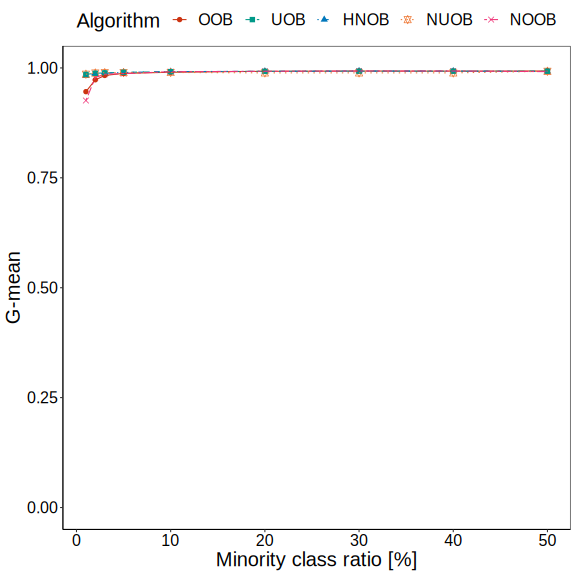
\includegraphics[width=7cm]{figures/imbalance_plot_G-mean.png}}
    \qquad
    \subfloat{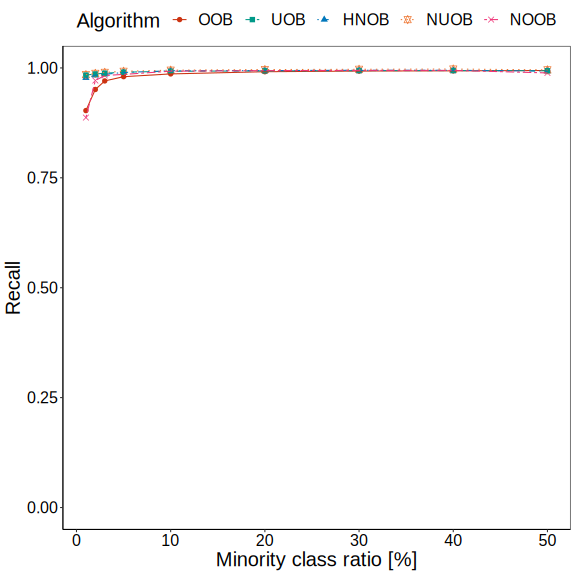
\includegraphics[width=7cm]{figures/imbalance_plot_Recall.png}}
    \caption{Porównanie jakości klasyfikacji dla różnych wartości współczynników niezbalansowania}\label{Figure:StaticImbalance}
\end{figure}

\newpage

\begin{table}[ht]
\centering\small%
\renewcommand{\arraystretch}{1.5} 
\begin{tabular}{c c c c c c}
\toprule
Imbalance Ratio & OB & UOB & OOB & NUOB & NOOB \\
\midrule
1\% & 0.807 & 0.985 & 0.945 & 0.985 & 0.925 \\
2\% & 0.913 & 0.987 & 0.972 & 0.988 & 0.978 \\
3\% & 0.935 & 0.988 & 0.982 & 0.989 & 0.985 \\
5\% & 0.962 & 0.990 & 0.987 & 0.989 & 0.987 \\
10\% & 0.977 & 0.991 & 0.990 & 0.989 & 0.991 \\
20\% & 0.988 & 0.992 & 0.992 & 0.988 & 0.992 \\
\bottomrule
\end{tabular}
\caption{Porównanie jakości klasyfikacji miary \textit{G-mean} w zależności od wartości współczynnika niezbalansowania}\label{Tab:ImbalanceRatio}
\end{table}

\noindent \textbf{Dryf pojęć ze zmianą współczynnika niezbalansowania}\\

\noindent Drugim z analizowanych czynników trudności będzie dryf pojęć ze zmianą współczynnika niezbalansowania (\textit{Im}). W przypadku wystąpienia dryfu związanego ze zmniejszeniem wartości współczynnika niezbalansowania można zaobserwować podobną sytuację, co przy analizie strumieni ze stałą wartością. Wszystkie klasyfikatory radzą sobie bardzo dobrze ze zmianami, jeśli przed wystąpieniem zjawiska dryfu współczynnik niezbalansowania wynosił przynajmniej 20\%. Sytuacja ta zaczyna się zmieniać, gdy przykładów do nauki było mniej przed wystąpieniem dryfu. Można zauważyć, że dla tych przypadków najgorzej radził sobie algorytm \textit{OB}. Pozostałe algorytmy także zaliczyły lekki spadek jakości klasyfikacji, jednak nadal utrzymywał się on koło wartości 0.98 dla miary \textit{G-mean} dla najlepszych algorytmów \textit{UOB} oraz \textit{NUOB}.

Sytuacja zmienia się w przypadku zaobserwowania dryfu związane ze zwiększeniem się wartości współczynnika niezbalansowania. Największy spadek jakości klasyfikacji dla algorytmów można zaobserwować dla przypadku, gdzie przed wystąpieniem dryfu pojęć liczba przykładów z klasy mniejszościowej stanowi zaledwie 1\% wszystkich przykładów. Najgorzej spisującym się algorytmem w tym przypadku był \textit{OB}, lekki spadek widoczny jest także dla algorytmów \textit{NOOB} oraz \textit{OOB}.

Podsumowując, zaprezentowane algorytmy w większości przypadków radzą sobie bardzo dobrze ze zjawiskiem zmiany współczynnika niezbalansowania. Dla najbardziej wymagających scenariuszy, gdzie przykładów z klasy mniejszościowej przed dryfem jest bardzo mało, można zaobserwować lekkie spadki jakości klasyfikacji dla średniej wartości miary \textit{G-mean}, jednak spadki te nie są bardzo duże. Zbiorowe wyniki klasyfikacji zostały przedstawione na rysunku \ref{Figure:DriftImbalance}. Jak można zauważyć na ilustracji \ref{Figure:StaticIm1_Im60} przedstawiającej scenariusz \textit{StaticIm1+Im60}, głównym problemem w procesie uczenia jest mała ilość przykładów z klasy mniejszościowej. Po wystąpieniu dryfu można zaobserwować, że jakość klasyfikacji wzrasta i utrzymuje się na poziomie wartości 0.99 dla obu badanych miar. W przypadku scenariuszy charakteryzujących się spadkiem współczynnika niezbalansowania (zaprezentowanych na ilustracji \ref{Figure:StaticIm10_Im1}), tak jak się można  spodziewać, widoczne jest obniżenie jakości klasyfikacji dla algorytmów po wystąpieniu dryfu. Mimo chwilowego spadku wszystkie algorytmy reagują odpowiednio na zmiany i ostatecznie wracają do poziomu, który występował przed dryfem.

\begin{figure}[h]
    \centering
    \includegraphics[width=7cm]{figures/algorithms_legend.JPG}
\end{figure}

\vspace{-1.2cm}

\begin{figure}[h]
    \centering
    \subfloat{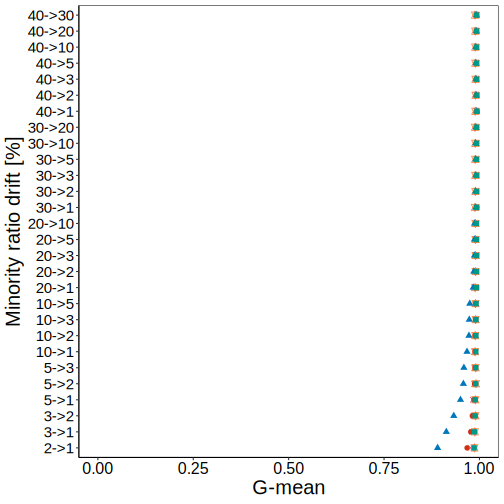
\includegraphics[width=7cm]{figures/dynamic_decreasing_plot_G-mean.png}}
    \qquad
    \subfloat{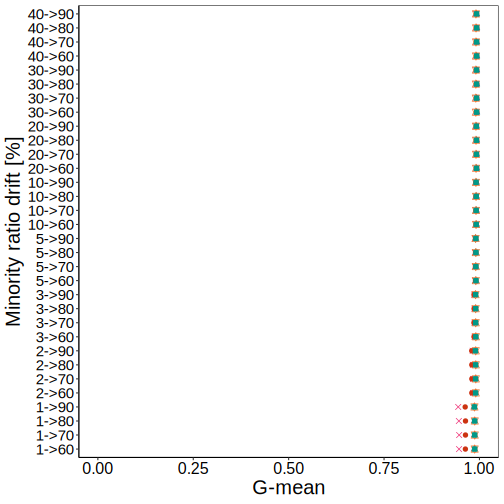
\includegraphics[width=7cm]{figures/dynamic_increasing_plot_G-mean.png}}
    \caption{Porównanie jakości klasyfikacji przy zmianie współczynnika niezbalansowania podczas zjawiska dryfu}\label{Figure:DriftImbalance}
\end{figure}

\begin{figure}[h]
    \centering
    \subfloat{\includegraphics[width=7cm]{figures/staticim1_im60_gmean.png}}
    \qquad
    \subfloat{\includegraphics[width=7cm]{figures/staticim1_im60_recall.png}}
    \caption{Wykresy liniowe miar \textit{G-mean} oraz \textit{Recall} dla strumienia \textit{StaticIm1+Im60}}\label{Figure:StaticIm1_Im60}
\end{figure}

\newpage

\begin{figure}[h]
    \centering
    \subfloat{\includegraphics[width=7cm]{figures/staticim10_im1_gmean.png}}
    \qquad
    \subfloat{\includegraphics[width=7cm]{figures/staticim5_im1_gmean.png}}
    \caption{Wykresy liniowe miary \textit{G-mean} dla strumieni \textit{StaticIm10+Im1} (po lewej) oraz \textit{StaticIm5+Im1} (po prawej)}\label{Figure:StaticIm10_Im1}
\end{figure}

\vspace{0.7cm}

\noindent \textbf{Zmiana rozkładu klasy mniejszościowej}\\

\noindent Trzecim z analizowanych czynników trudności będzie zmiana rozkładu klasy mniejszościowej. Czynnik ten powiązany jest ze zmianą pozycji skupisk przykładów klasy mniejszościowej. Obejmuje następujące scenariusze:

\begin{itemize}
    \item Podział skupiska przykładów klasy mniejszościowej na mniejsze grupy przykładów (\textit{Split})
    \item Przesuwanie się skupisk w przestrzeni atrybutów (\textit{Move})
    \item Połączenie grup przykładów klasy mniejszościowej w jedno większe skupisko (\textit{Merge})
\end{itemize}

\begin{figure}[h]
    \centering
    \subfloat{\includegraphics[width=7cm]{figures/split5_gmean.png}}
    \qquad
    \subfloat{\includegraphics[width=7cm]{figures/split5_recall.png}}
    \caption{Wykresy liniowe miar \textit{G-mean} oraz \textit{Recall} dla strumienia \textit{Split5}}\label{Figure:Split5}
\end{figure}

\noindent W przypadku scenariusza związanego z podziałem skupiska można zauważyć spadek w jakości klasyfikacji w trakcie występowania dryfu pojęć. Jak można zauważyć większość klasyfikatorów zachowała się bardzo podobnie. Po zaobserwowanym spadku widoczny jest wzrost, który świadczy o tym, że algorytmy przystosowały się odpowiednio do zmian, które zaszły w badanym strumieniu. Identyczny efekt można zaobserwować dla scenariusza, gdy grupy przykładów przemieszczają się w przestrzeni atrybutów. W trakcie przemieszczania widoczny jest spadek wartości badanych miar, natomiast po przemieszczeniu klasyfikatory odpowiednio przystosowują się do zmian, co skutkuje wzrostem jakości klasyfikacji. Podobną sytuację można zaobserwować w przypadku połączenia grup przykładów w większe skupisko, co zostało przedstawione na rysunku \ref{Figure:Join5}.

\begin{figure}[h]
    \centering
    \subfloat{\includegraphics[width=7cm]{figures/join5_gmean.png}}
    \qquad
    \subfloat{\includegraphics[width=7cm]{figures/join5_recall.png}}
    \caption{Wykresy liniowe miar \textit{G-mean} oraz \textit{Recall} dla strumienia \textit{Merge5}}\label{Figure:Join5}
\end{figure}

\begin{figure}[h]
    \centering
    \includegraphics[width=7cm]{figures/algorithms_legend.JPG}
\end{figure}

\vspace{-1.2cm}

\begin{figure}[h]
    \centering
    \subfloat{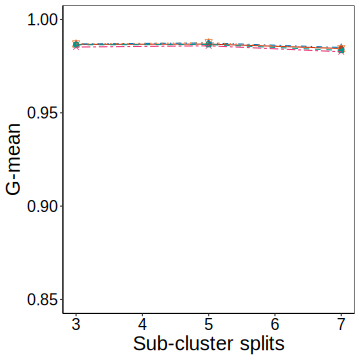
\includegraphics[width=4cm]{figures/Split_plot_G-mean.png}}
    \qquad
    \subfloat{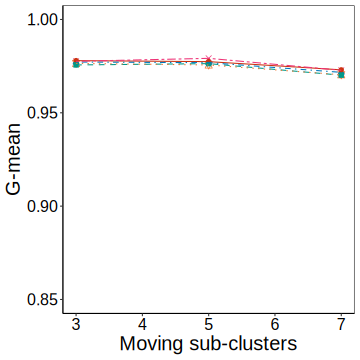
\includegraphics[width=4cm]{figures/Move_plot_G-mean.png}}
    \qquad
    \subfloat{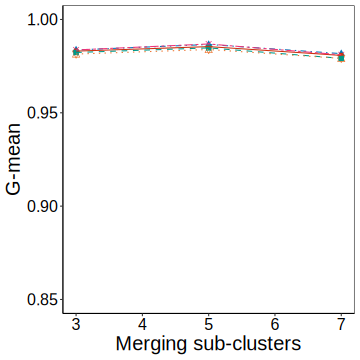
\includegraphics[width=4cm]{figures/join_plot_G-mean.png}}
    \caption{Porównanie jakości klasyfikacji przy zmianie liczby skupisk przykładów klasy mniejszościowej}\label{Figure:ChangeComposition}
\end{figure}

\noindent Podsumowując, wszystkie przedstawione algorytmy radziły sobie identycznie z problemem zmiany rozkładu klasy mniejszościowej. Jak można zauważyć na rysunku \ref{Figure:ChangeComposition} większa lub mniejsza liczba skupisk nie wpływała znacząco na jakość klasyfikacji zaprezentowanych modeli. Każdy z klasyfikatorów po wystąpieniu dryfu pojęć był w stanie przystosować się do zmian, które zaszły w strumieniu i powrócić na wysoki poziom jakości klasyfikacji.

\newpage

\noindent \textbf{Napływ przykładów określonego typu}\\

\noindent Ostatnim z analizowanych czynników trudności będzie napływ przykładów określonego typu. W ramach tej analizy rozważone zostaną przykłady o typie brzegowym (\english{borderline}) oraz rzadkim (\english{rare}).

\begin{table}[ht]
\centering\small%
\renewcommand{\arraystretch}{1.5} 
\begin{tabular}{l c c c c c c}
\toprule
Configuration & N & OB & UOB & OOB & NUOB & NOOB \\
\midrule
Safe stream & 0\% & 0.992 & 0.992 & 0.993 & 0.992 & 0.991 \\
Borderline[N] & 20\% & 0.978 & 0.978 & 0.978 & 0.979 & 0.969 \\
& 40\% & 0.974 & 0.974 & 0.974 & 0.976 & 0.965 \\
& 60\% & 0.972 & 0.971 & 0.972 & 0.973 & 0.963 \\
& 80\% & 0.971 & 0.970 & 0.971 & 0.972 & 0.961 \\
& 100\% & 0.969 & 0.968 & 0.969 & 0.970 & 0.959 \\
Rare[N] & 20\% & 0.935 & 0.935 & 0.935 & 0.935 & 0.934 \\
& 40\% & 0.865 & 0.865 & 0.865 & 0.865 & 0.866 \\
& 60\% & 0.779 & 0.779 & 0.779 & 0.779 & 0.800 \\
& 80\% & 0.684 & 0.680 & 0.690 & 0.677 & 0.752 \\
& 100\% & 0.677 & 0.668 & 0.689 & 0.661 & 0.692 \\
\bottomrule
\end{tabular}
\caption{Porównanie jakości klasyfikacji miary \textit{G-mean} w zależności od napływu przykładów określonego typu. Wartości w tabeli zostały wyznaczone jako średnia wszystkich wyników obliczonych podczas oceny odpowiedniego strumienia}\label{Tab:BorderlineRare}
\end{table}

\noindent Na podstawie przedstawionej tabeli \ref{Tab:BorderlineRare} można zauważyć, że porównywane klasyfikatory bardzo dobrze radzą sobie z napływem przykładów typu \textit{borderline}. Niestety widoczny jest znaczący spadek klasyfikacji w przypadku napływu przykładów typu \textit{Rare}. Identyczny efekt można zaobserwować przy zestawieniu wyników miary \textit{Recall}. Z zaprezentowanych rezultatów można wyciągnąć wniosek, że algorytm \textit{NOOB} radzi sobie trochę lepiej z rozpoznawaniem przykładów rzadkich aniżeli pozostałe algorytmy. Potwierdzenie tej obserwacji można zobaczyć na rysunku \ref{Figure:Rare80}.

\newpage

\begin{figure}[h]
    \centering
    \includegraphics[width=12cm]{figures/rare80_gmean.png}
    \caption{Wykres liniowy miary \textit{G-mean} dla strumienia \textit{Rare80}}\label{Figure:Rare80}
\end{figure}

\begin{figure}[h]
    \centering
    \includegraphics[width=7cm]{figures/algorithms_legend.JPG}
\end{figure}

\vspace{-1.2cm}

\begin{figure}[h]
    \centering
    \subfloat{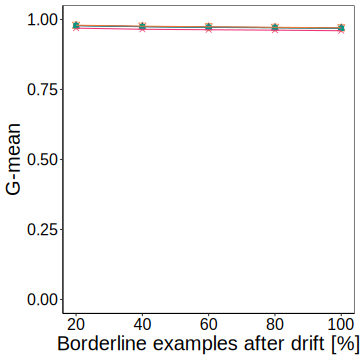
\includegraphics[width=7cm]{figures/borderline_plot_G-mean.png}}
    \qquad
    \subfloat{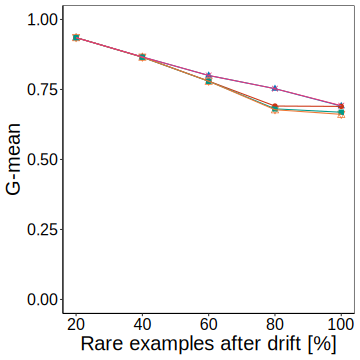
\includegraphics[width=7cm]{figures/rare_plot_G-mean.png}}
    \caption{Porównanie jakości klasyfikacji przy zmianie liczby przykładów określonego typu}\label{Figure:BorderlineRare}
\end{figure}

\noindent Podsumowując, wszystkie przedstawione algorytmy radzą sobie bardzo dobrze ze wzrostem przykładów typu \textit{Borderline}. Niestety w przypadku wzrostu elementów typu \textit{Rare} widoczny jest znaczący spadek jakości klasyfikacji. Jedynym wyróżniającym się algorytmem, który radził sobie lepiej od pozostałych z rozpoznawaniem przykładów rzadkich, był algorytm \textit{NOOB}, jednak nawet ten klasyfikator nie dał rady odpowiednio dostosować się do zmian i powrócić na swój początkowy poziom jakości klasyfikacji przed wystąpieniem dryfu.

\noindent \textbf{Porównanie statystyczne klasyfikatorów}\\

\noindent W ramach ostatniego punktu analizy klasyfikatorów pod kątem strumieni danych z jednym czynnikiem trudności, przeprowadzony zostanie test statystyczny rang Friedman'a, którego kontynuacją będzie przeprowadzenie testu Nemenyi jako testu \textit{post hoc}. Testy zostały przeprowadzone na poziomie istotności $\alpha$ = 0.05.

\begin{table}[ht]
\centering\small%
\setlength{\tabcolsep}{10pt} 
\renewcommand{\arraystretch}{1.5} 
\begin{tabular}{l l c c c c c c}
\toprule
Data stream set & Metric & OB & UOB & OOB & NUOB & NOOB & CD \\
\midrule
Static imbalance & G-mean & 3.82 & \textbf{2.00} & \textbf{2.29} & \textbf{3.29} & 3.59 & 1.51 \\
Class ratio changes & & 4.55 & \textbf{1.59} & 2.61 & 3.14 & 3.11 & 0.77 \\
Sub-cluster merge & & \textbf{2.67} & \textbf{3.83} & \textbf{2.33} & \textbf{3.17} & \textbf{3.00} & 2.68 \\
Sub-cluster move & & \textbf{2.67} & 4.83 & \textbf{1.33} & 4.17 & \textbf{2.00} & 2.68 \\
Sub-cluster split & & \textbf{2.17} & \textbf{4.50} & \textbf{2.17} & \textbf{2.00} & \textbf{4.17} & 2.68 \\
Borderline examples & & \textbf{1.70} & 4.00 & \textbf{2.40} & \textbf{2.60} & 4.30 & 2.01 \\
Rare examples & & \textbf{2.80} & 4.20 & \textbf{1.90} & 4.00 & \textbf{2.10} & 2.01 \\
Static imbalance & Recall & 4.35 & \textbf{2.41} & 3.35 & \textbf{1.00} & 3.88 & 1.51 \\
Class ratio changes & & 4.88 & 2.17 & 3.59 & \textbf{1.00} & 3.36 & 0.77 \\
Sub-cluster merge & & \textbf{2.67} & \textbf{3.67} & \textbf{2.67} & \textbf{1.00} & 5.00 & 2.68 \\
Sub-cluster move & & \textbf{3.17} & \textbf{3.17} & \textbf{2.67} & \textbf{1.00} & 5.00 & 2.68 \\
Sub-cluster split & & \textbf{2.50} & \textbf{2.50} & 4.00 & \textbf{1.00} & 5.00 & 2.68 \\
Borderline examples & & \textbf{2.70} & 3.80 & \textbf{2.50} & \textbf{1.00} & 5.00 & 2.01 \\
Rare examples & & \textbf{3.90} & \textbf{3.80} & \textbf{2.80} & \textbf{2.10} & \textbf{2.40} & 2.01 \\
\bottomrule
\end{tabular}
\caption{Wyniki przeprowadzonych testów statystycznych dla pojedynczych czynników trudności}\label{Tab:SingleDriftFriedman}
\end{table}

\noindent W tabeli \ref{Tab:SingleDriftFriedman} zestawione zostały wyniki przeprowadzonych testów statystycznych. Interpretacja wyników otrzymanych w tabeli jest następująca - im mniejsza wartość rangi dla danego algorytmu tym lepsze rezultaty osiągało dane podejście. Pogrubione zostały najlepsze wyniki dla określonych zbiorów danych oraz wyniki, które okazały się nie być statystycznie różne od najlepszego wyniku. Kolumna \textit{CD} oznacza odległość krytyczną (\english{critical distance}), na podstawie której to wartości można określić czy dwa otrzymane wyniki są od siebie statystycznie różne czy nie (na zadanym poziomie istotności). Na podstawie otrzymanych rezultatów możliwe jest określenie rankingu algorytmów pod kątem danej miary:

\begin{itemize}
    \item \textit{G-mean} - OOB $\succ$ OB $\succ$ UOB, NUOB, NOOB
    \item \textit{Recall} - NUOB $\succ$ OB, UOB $\succ$ OOB $\succ$ NOOB
\end{itemize}

\noindent Najlepszym algorytmem pod kątem miary \textit{G-mean}, dla strumieni danych charakteryzujących się występowaniem jednego czynnika trudności, okazał się algorytm \textit{OOB}, co jest niekorzystnym wynikiem, gdyż pokazuje to, że zaproponowane rozszerzenia nie radzą sobie najlepiej. Obserwacja ta pozostawia pole do poprawy oraz dalszej analizy względem zaproponowanych algorytmów. Pod kątem miary \textit{Recall} najlepszy był nowo zaprezentowany algorytm \textit{NUOB}.

\subsection{Data streams with pairs of factors}

\noindent W niniejszej sekcji zaprezentowane algorytmy zostaną przetestowane pod kątem jakości klasyfikacji na strumieniach danych z dwoma czynnikami trudności (\english{pairs of factors}). Jak się okazało, na podstawie wyników poprzedniej sekcji, najbardziej wymagającym czynnikiem, z którym algorytmy miały największe problemy, był napływ przykładów typu \textit{Rare}. Bardzo podobnie sytuacja wygląda w przypadku analizy par czynników, które mogą wystąpić w strumieniu. Jeżeli jednym z tych czynników jest napływ rzadkich przykładów to jakość klasyfikacji jest zdecydowanie niższa aniżeli gdy dokonujemy analizy strumienia zawierającego inne własności. Odwzorowanie tej sytuacji można zobaczyć na rysunkach \ref{Figure:Split5Pairs} oraz \ref{Figure:PairsFactors}.

\begin{figure}[h]
    \centering
    \subfloat{\includegraphics[width=7cm]{figures/split5im10_gmean.png}}
    \qquad
    \subfloat{\includegraphics[width=7cm]{figures/split5rare80_gmean.png}}
    \caption{Wykresy liniowe miary \textit{G-mean} dla strumieni \textit{Split5+Im10} (po lewej) oraz \textit{Split5+Rare80} (po prawej)}\label{Figure:Split5Pairs}
\end{figure}

\begin{figure}[h]
    \centering
    \subfloat{\includegraphics[width=7cm]{figures/im1borderline80_gmean.png}}
    \qquad
    \subfloat{\includegraphics[width=7cm]{figures/split5rare60_gmean.png}}
    \caption{Wykresy liniowe miary \textit{G-mean} dla strumieni \textit{Im1+Borderline80} (po lewej) oraz \textit{Split5+Rare60} (po prawej)}\label{Figure:PairsFactors}
\end{figure}

\noindent Podobnie, jak to można było zauważyć we wcześniejszej sekcji, algorytm NOOB radzi sobie trochę lepiej z rozpoznawaniem przykładów rzadkich w porównaniu do innych algorytmów. Aby potwierdzić tę tezę na innych scenariuszach, zdecydowano się zestawić wyniki wszystkich algorytmów na najbardziej wymagających strumieniach danych. Otrzymane wyniki widoczne są na rysunku \ref{Figure:PairsComparison}.

\begin{figure}[h]
    \centering
    \includegraphics[width=7cm]{figures/algorithms_legend.JPG}
\end{figure}

\vspace{-1.2cm}

\begin{figure}[h]
    \centering
    \subfloat{\includegraphics[width=7cm]{figures/pair_plot_G-mean.png}}
    \qquad
    \subfloat{\includegraphics[width=7cm]{figures/pair_plot_Recall.png}}
    \caption{Porównanie jakości klasyfikacji na najbardziej wymagających strumieniach danych zawierających dwa czynniki trudności}\label{Figure:PairsComparison}
\end{figure}

\noindent Jak można zauważyć na ilustracji \ref{Figure:PairsComparison} algorytm \textit{NOOB} radzi sobie zdecydowanie lepiej od pozostałych algorytmów na najbardziej wymagających strumieniach danych. Przykładowo dla strumienia \textit{Im1+Rare80} wartość miary \textit{G-mean} dla algorytmu \textit{NOOB} wynosi około 0.8, podczas gdy dla pozostałych algorytmów jest to wartość około 0.65. Podobne rezultaty można zaobserwować dla tego samego strumienia dla miary \textit{Recall}. Dla podejścia \textit{NOOB} jest to wartość około 0.75, a dla pozostałych algorytmów około 0.5. Analogiczną sytuację można zaobserwować na strumieniu \textit{Im10+Rare60} lub \textit{Im10+Rare40}. Należy także zwrócić uwagę na obserwację dotyczącą tego, że algorytmy \textit{OB} oraz \textit{OOB} kompletnie nie radzą sobie z klasyfikacją trudnych strumieni danych - na strumieniu \textit{Im1+Rare100} wartość miar \textit{G-mean} oraz \textit{Recall} oscyluje koło wartości 0.4.

Podobnie jak w poprzedniej sekcji przeprowadzono porównanie statystyczne klasyfikatorów z wykorzystaniem testu statystycznego rang Friedman'a oraz testu Nemenyi na poziomie istotności $\alpha$ = 0.05.

\newpage

\begin{table}[ht]
\centering\small%
\setlength{\tabcolsep}{10pt} 
\renewcommand{\arraystretch}{1.5} 
\begin{tabular}{l l c c c c c c}
\toprule
Data stream set & Metric & OB & UOB & OOB & NUOB & NOOB & CD \\
\midrule
Imbalance + Move & G-mean & 5.00 & \textbf{2.33} & \textbf{2.75} & \textbf{2.67} & \textbf{2.25} & 1.82 \\
Imbalance + Merge  & & 5.00 & \textbf{1.75} & \textbf{3.08} & \textbf{2.25} & \textbf{2.92} & 1.82 \\
Imbalance + Split  & & 5.00 & \textbf{2.11} & 3.50 & \textbf{2.00} & \textbf{2.39} & 1.47 \\
Imbalance + Borderline  & & 5.00 & \textbf{2.42} & 3.38 & \textbf{1.68} & \textbf{2.52} & 0.97 \\
Imbalance + Rare  & & 4.85 & 2.88 & 3.10 & 2.95 & \textbf{1.23} & 0.97 \\
Split + Borderline  & & 4.36 & \textbf{2.44} & 3.22 & \textbf{2.14} & \textbf{2.84} & 0.87 \\
Split + Rare  & & 4.54 & 2.94 & 3.24 & 2.76 & \textbf{1.52} & 0.87 \\
Imbalance + Move & Recall & 5.00 & \textbf{2.17} & 3.83 & \textbf{1.33} & \textbf{2.67} & 1.82 \\
Imbalance + Merge  & & 5.00 & \textbf{2.00} & 3.83 & \textbf{1.42} & \textbf{2.75} & 1.82 \\
Imbalance + Split  & & 5.00 & \textbf{2.06} & 3.83 & \textbf{1.33} & \textbf{2.78} & 1.47 \\
Imbalance + Borderline  & & 5.00 & 2.52 & 3.88 & \textbf{1.35} & \textbf{2.25} & 0.97 \\
Imbalance + Rare  & & 5.00 & 2.73 & 3.83 & \textbf{2.10} & \textbf{1.35} & 0.97 \\
Split + Borderline  & & 4.52 & 2.60 & 3.68 & \textbf{1.60} & 2.60 & 0.87 \\
Split + Rare  & & 4.50 & \textbf{2.72} & 3.76 & \textbf{2.16} & \textbf{1.86} & 0.87 \\
\bottomrule
\end{tabular}
\caption{Wyniki przeprowadzonych testów statystycznych dla par czynników trudności}\label{Tab:DoubleDriftFriedman}
\end{table}

\noindent W tabeli \ref{Tab:DoubleDriftFriedman} zestawione zostały wyniki przeprowadzonych testów statystycznych. Interpretacja wyników otrzymanych w tabeli jest następująca - im mniejsza wartość rangi dla danego algorytmu tym lepsze rezultaty osiągało dane podejście. Pogrubione zostały najlepsze wyniki dla określonych zbiorów danych oraz wyniki, które okazały się nie być statystycznie różne od najlepszego wyniku. Na podstawie otrzymanych rezultatów możliwe jest określenie rankingu algorytmów pod kątem danej miary:

\begin{itemize}
    \item \textit{G-mean} - NOOB $\succ$ UOB, NUOB $\succ$ OOB $\succ$ OB
    \item \textit{Recall} - NUOB $\succ$ NOOB $\succ$ UOB $\succ$ OB, OOB
\end{itemize}

\noindent Najlepszym algorytmem pod kątem miary \textit{G-mean}, dla strumieni charakteryzujących się występowaniem par czynników trudności, okazał się \textit{NOOB}. Pod kątem miary \textit{Recall} ponownie najlepszy był algorytm \textit{NUOB}. Warto odnotować, że algorytmy \textit{OB} oraz \textit{OOB} osiągnęły słabe wyniki w porównaniu do innych algorytmów, co sugeruje, że niekoniecznie radzą sobie ze złożonymi instancjami strumieni danych.

\subsection{Complex scenarios}

\noindent W ramach tej części zaprezentowane algorytmy zostaną przetestowane pod kątem jakości klasyfikacji na strumieniach danych z wieloma czynnikami trudności (\english{complex scenarios}). Podobnie jak to było przy ocenie strumieni z dwoma czynnikami trudności, tak tutaj największy wpływ na jakość klasyfikacji ma napływ elementów rzadkich. Z takimi scenariuszami radzi sobie najlepiej algorytm \textit{NOOB}, czego odzwierciedlenie można zobaczyć na rysunku \ref{Figure:ComlexScenario}.

\newpage

\begin{figure}[h]
    \centering
    \subfloat{\includegraphics[width=7cm]{figures/complex_scenario_gmean.png}}
    \qquad
    \subfloat{\includegraphics[width=7cm]{figures/complex_scenario_recall.png}}
    \caption{Wykresy liniowe miar \textit{G-mean} oraz \textit{Recall} dla strumienia \textit{StaticIm10+Split5+Im1+Rare80}}\label{Figure:ComlexScenario}
\end{figure}

\noindent W celach porównawczych dokonano zestawienia wyników algorytmów na strumieniach danych, które najbardziej wpływają na spadek jakości klasyfikacji. Otrzymane wyniki widoczne są na rysunku \ref{Figure:ComplexComparison}.

\begin{figure}[h]
    \centering
    \includegraphics[width=7cm]{figures/algorithms_legend.JPG}
\end{figure}

\vspace{-1.2cm}

\begin{figure}[h]
    \centering
    \subfloat{\includegraphics[width=7cm,height=9cm]{figures/complex_plot_G-mean.png}}
    \qquad
    \subfloat{\includegraphics[width=7cm,height=9cm]{figures/complex_plot_Recall.png}}
    \caption{Porównanie jakości klasyfikacji na najbardziej wymagających strumieniach danych zawierających wiele czynników trudności}\label{Figure:ComplexComparison}
\end{figure}

\noindent Podobnie jak to było przy analizie strumieni z dwoma czynnikami trudności tak też tutaj można zauważyć, że algorytm \textit{NOOB} radzi sobie zdecydowanie lepiej od pozostałych algorytmów na najbardziej wymagających strumieniach danych. Obserwację tę potwierdzają wyniki otrzymane podczas analizy takich scenariuszy jak: \textit{StaticIm10+Split5+Im1+Rare100}, \textit{Split5+Im1Rare80}, \textit{StaticIm10+Split5+Im1+Rare60} - wyniki oscylującą w okolicy wartości 0.8 dla miary \textit{G-mean} oraz 0.7 dla miary \textit{Recall}. Należy także zwrócić uwagę, że drugi z zaproponowanych algorytmów \textit{NUOB} także daje sobie radę na analizowanych strumieniach. Wyróżniającymi się scenariuszami, pod kątem analizy obu miar, w tym przypadku były: \textit{Split5+Im10+Rare100}, \textit{Split5+Im1+Borderline40+Rare40}, \textit{Split5+Im1+Rare60}. Algorytmem, który charakteryzuje się najniższą jakością klasyfikacji, jest algorytm \textit{OB}, co potwierdza teorię, że poprzez losowanie z rozkładu Possiona z parametrem $\lambda$ = 1, algorytm ten nie będzie sobie w stanie odpowiednio poradzić na złożonych strumieniach danych.

W ramach tej sekcji przeprowadzono również porównanie statystyczne klasyfikatorów, jednak ze względu na mnogość kombinacji, zaprezentowane zostaną wyniki zbiorcze:

\begin{itemize}
    \item Na strumieniach danych zawierających co najmniej dwa czynniki trudności - \textit{multiple}
    \item Na wszystkich strumieniach danych - \textit{all}
\end{itemize}

\begin{table}[ht]
\centering\small%
\setlength{\tabcolsep}{10pt} 
\renewcommand{\arraystretch}{1.5} 
\begin{tabular}{l l c c c c c c}
\toprule
Data stream set & Metric & OB & UOB & OOB & NUOB & NOOB & CD \\
\midrule
Multiple & G-mean & 4.60 & 2.69 & 3.27 & \textbf{2.30} & \textbf{2.14} & 0.43 \\
All  & & 4.39 & \textbf{2.56} & 2.99 & \textbf{2.58} & \textbf{2.48} & 0.31 \\
Multiple & Recall & 4.67 & 2.61 & 3.76 & \textbf{1.79} & \textbf{2.17} & 0.43\\
All  & & 4.58 & 2.60 & 3.62 & \textbf{1.53} & 2.67 & 0.31 \\
\bottomrule
\end{tabular}
\caption{Wyniki przeprowadzonych testów statystycznych}\label{Tab:ComplexFriedman}
\end{table}

\noindent W tabeli \ref{Tab:ComplexFriedman} zestawione zostały wyniki przeprowadzonych testów statystycznych. Pod kątem kryterium przetwarzania na strumieniach danych zawierających co najmniej dwa czynniki trudności można wyszczególnić algorytmy: \textit{NUOB} oraz \textit{NOOB}. Biorąc pod uwagę wszystkie strumienie danych najlepiej prezentowały się algorytmy: \textit{UOB}, \textit{NUOB} oraz \textit{NOOB}.

\subsection{Podsumowanie}

\noindent W ramach niniejszego podrozdziału dokonano porównania algorytmów \textit{OB}, \textit{UOB}, \textit{OOB} z nowymi propozycjami algorytmów przetwarzania strumieniowego \textit{NUOB} oraz \textit{NOOB}. Przeprowadzona analiza została dokonana z podziałem na strumienie z jednym czynnikiem trudności (\english{single factors}), z dwoma czynnikami trudności (\english{pairs of factors}) oraz wieloma czynnikami trudności (\english{complex scenarios}).

Przeprowadzone testy na strumieniach z jednym czynnikiem trudności wykazały podobieństwo zaproponowanych algorytmów do już istniejących podejść pod kątem osiąganych wyników. Na wielu kryteriach otrzymane wyniki nie były statystycznie różne od najlepszych wyników. Pod kątem miary \textit{Recall} algorytm \textit{NUOB} okazał się najlepszy spośród wszystkich testowanych podejść.

Sytuacja lekko zmieniła się po przeprowadzeniu testów dla strumieni danych z dwoma i więcej czynnikami trudności. Nowo zaproponowane algorytmy \textit{NUOB} oraz \textit{NOOB} często osiągały najlepsze rezultaty na określonych scenariuszach. Przeprowadzone testy statystyczne także potwierdziły te obserwacje. Pod kątem miary \textit{G-mean} najlepszy okazał się algorytm \textit{NOOB}, a zaraz za nim kolejne miejsce zajął klasyfikator \textit{NUOB}. W przypadku miary \textit{Recall} sytuacja odwróciła się - najlepszy okazał się \textit{NUOB}, a zaraz za nim był \textit{NOOB}.

Wyniki przeprowadzonych testów pokazują, że zaproponowane w niniejszej pracy algorytmy charakteryzują się dobrymi wynikami w porównaniu do istniejących podejść, co może być potwierdzeniem realizacji założonego celu rozprawy.

\section{Hybrid Neighbourhood Online Bagging}

\noindent Przedstawiany w tej sekcji algorytm \textit{Hybrid Neighbourhood Online Bagging} składa się z dwóch klasyfikatorów składowych: \textit{Neighbourhood Undersampling Online Bagging} oraz \textit{Neighbourhood Oversampling Online Bagging}. Parametry używane w wymienionych algorytmach mają takie same wartości jak przy porównaniu, które zostało wykonane w ramach sekcji \ref{Section:AlgorithmsComparison}. Sprawa ma się podobnie dla algorytmów \textit{Oversampling Online Bagging} oraz \textit{Undersampling Online Bagging}, które także wykorzystują te same wartości parametrów, co przedstawione w sekcji wcześniejszej.

\subsection{Data streams with single factors}

\noindent Przedstawiany algorytm \textit{Hybrid Neighbourhood Online Bagging (HNOB)} charakteryzuje się tym, że stara się dopasować do aktualnie najlepszego pod względem miary \textit{G-mean} klasyfikatora składowego. Oznacza to, że bardzo często ten algorytm osiąga bardzo podobne wyniki, co lepsza z wersji algorytmów \textit{NUOB}, \textit{NOOB}. Efekt ten można m.in. zobaczyć na rysunkach \ref{Figure:Split7} oraz \ref{Figure:BorderlineRareHNOB}, gdzie podczas dryfu algorytm \textit{HNOB} dopasowuje się do aktualnie najlepszego algorytmu \textit{NUOB} i osiąga praktycznie identyczne wyniki.

\begin{figure}[h]
    \centering
    \includegraphics[width=11cm]{figures/split7_gmean.png}
    \caption{Wykres liniowy miary \textit{G-mean} dla strumienia \textit{Split7}}\label{Figure:Split7}
\end{figure}

\newpage

\begin{figure}[h]
    \centering
    \subfloat{\includegraphics[width=7cm]{figures/borderline60_hnob_gmean.png}}
    \qquad
    \subfloat{\includegraphics[width=7cm]{figures/rare60_hnob_gmean.png}}
    \caption{Wykresy liniowe miary \textit{G-mean} dla strumieni \textit{Borderline60} (po lewej) oraz \textit{Rare60} (po prawej)}\label{Figure:BorderlineRareHNOB}
\end{figure}

\noindent Aby ocenić jak radzi sobie algorytm \textit{HNOB} na strumieniach danych z jednym czynnikiem trudności, zdecydowano się przeprowadzić testy statystyczne z wykorzystaniem testu rang Friedman'a, którego kontynuacją będzie przeprowadzenie testu Nemenyi jako testu \textit{post hoc}. Wszystkie rezultaty zostały zweryfikowane na poziomie istotności $\alpha$ = 0.05.

\begin{table}[ht]
\centering\small%
\setlength{\tabcolsep}{10pt} 
\renewcommand{\arraystretch}{1.5} 
\begin{tabular}{l l c c c c c c}
\toprule
Data stream set & Metric & HNOB & UOB & OOB & NUOB & NOOB & CD \\
\midrule
Static imbalance & G-mean & \textbf{3.06} & \textbf{2.06} & \textbf{2.65} & \textbf{3.29} & 3.94 & 1.51 \\
Class ratio changes & & 2.70 & \textbf{1.84} & 3.25 & 3.47 & 3.73 & 0.77 \\
Sub-cluster merge & & \textbf{2.17} & \textbf{3.83} & \textbf{2.63} & \textbf{3.00} & \textbf{3.33} & 2.68 \\
Sub-cluster move & & \textbf{1.50} & 4.83 & \textbf{1.83} & \textbf{4.17} & \textbf{2.67} & 2.68 \\
Sub-cluster split & & \textbf{1.67} & 4.50 & \textbf{2.33} & \textbf{2.33} & \textbf{4.17} & 2.68 \\
Borderline examples & & \textbf{2.50} & \textbf{3.80} & \textbf{2.10} & \textbf{2.50} & \textbf{4.10} & 2.01 \\
Rare examples & & \textbf{2.30} & \textbf{3.90} & \textbf{2.50} & \textbf{4.00} & \textbf{2.30} & 2.01 \\
Static imbalance & Recall & 3.24 & 2.59 & 3.82 & \textbf{1.00} & 4.35 & 1.51 \\
Class ratio changes & & 2.64 & 2.63 & 4.48 & \textbf{1.02} & 4.23 & 0.77 \\
Sub-cluster merge & & \textbf{3.00} & \textbf{3.33} & \textbf{2.67} & \textbf{1.00} & 5.00 & 2.68 \\
Sub-cluster move & & 3.83 & \textbf{2.83} & \textbf{2.33} & \textbf{1.00} & 5.00 & 2.68 \\
Sub-cluster split & & \textbf{2.83} & \textbf{3.67} & \textbf{2.50} & \textbf{1.00} & 5.00 & 2.68 \\
Borderline examples & & \textbf{3.00} & 3.40 & \textbf{2.60} & \textbf{1.00} & 5.00 & 2.01 \\
Rare examples & & \textbf{2.20} & \textbf{4.00} & \textbf{3.40} & \textbf{2.50} & \textbf{2.90} & 2.01 \\
\bottomrule
\end{tabular}
\caption{Wyniki przeprowadzonych testów statystycznych dla pojedynczych czynników trudności}\label{Tab:SingleDriftFriedmanHNOB}
\end{table}

\noindent W tabeli \ref{Tab:SingleDriftFriedmanHNOB} przedstawione zostały wyniki przeprowadzonych testów statystycznych. Pogrubione zostały najlepsze wyniki dla określonych zbiorów danych oraz wyniki, które okazały się nie być statystycznie różne od najlepszego wyniku. Na podstawie otrzymanych rezultatów możliwe jest określenie rankingu algorytmów pod kątem danej miary:

\begin{itemize}
    \item \textit{G-mean} - HNOB, OOB, NUOB $\succ$ UOB, NOOB
    \item \textit{Recall} - NUOB $\succ$ OOB $\succ$ HNOB, UOB $\succ$ NOOB
\end{itemize}

\subsection{Data streams with pairs of factors}

\noindent W przypadku analizy strumieni danych z dwoma czynnikami trudności można się spodziewać, że algorytm hybrydowy poradzi sobie lepiej aniżeli przy analizie strumieni danych z jednym czynnikiem trudności. Jest to spowodowane faktem, że wcześniejsza analiza wykazała, że najlepszymi algorytmami były \textit{NOOB} oraz \textit{NUOB}. Algorytm hybrydowy powinien zaaplikować zalety obu tych klasyfikatorów w swoim działaniu. Aby zweryfikować tę tezę, zestawiono wyniki wszystkich algorytmów na najbardziej wymagających strumieniach danych. Otrzymane wyniki widoczne są na rysunku \ref{Figure:PairsComparisonHNOB}.

\begin{figure}[h]
    \centering
    \subfloat{\includegraphics[width=7cm]{figures/im10rare100_hnob_gmean.png}}
    \qquad
    \subfloat{\includegraphics[width=7cm]{figures/split5rare80_hnob_gmean.png}}
    \caption{Wykresy liniowe miary \textit{G-mean} dla strumieni \textit{Im10+Rare100} (po lewej) oraz \textit{Split5+Rare80} (po prawej)}\label{Figure:PairsFactorsHNOB}
\end{figure}

\begin{figure}[h]
    \centering
    \subfloat{\includegraphics[width=7cm]{figures/borderline40rare80_hnob_gmean.png}}
    \qquad
    \subfloat{\includegraphics[width=7cm]{figures/split5borderline80_hnob_gmean.png}}
    \caption{Wykresy liniowe miary \textit{G-mean} dla strumieni \textit{Borderline40+Rare40} (po lewej) oraz \textit{Split5+Borderline80} (po prawej)}
\end{figure}

\newpage

\begin{figure}[h]
    \centering
    \includegraphics[width=7cm]{figures/algorithms_legend_hnob.JPG}
\end{figure}

\vspace{-1.2cm}

\begin{figure}[h]
    \centering
    \subfloat{\includegraphics[width=7cm]{figures/pair_plot_G-mean_HNOB.png}}
    \qquad
    \subfloat{\includegraphics[width=7cm]{figures/pair_plot_Recall_HNOB.png}}
    \caption{Porównanie jakości klasyfikacji na najbardziej wymagających strumieniach danych zawierających dwa czynniki trudności}\label{Figure:PairsComparisonHNOB}
\end{figure}

\noindent Jak można zauważyć na ilustracji \ref{Figure:PairsComparisonHNOB} wysunięta teza okazała się prawdziwa w przypadku scenariuszy analizowanych pod kątem miary \textit{G-mean}. Algorytm hybrydowy osiąga rezultaty bardzo zbliżone do aktualnie najlepszego algorytmu. Można to zaobserwować w przypadku analizy takich scenariuszy, jak np. \textit{Im10+Rare40}, \textit{Im10+Rare60}, \textit{Split5+Rare60}. Sytuacja zmienia się trochę dla niektórych przykładów strumieni pod kątem miary \textit{Recall}. Dla większości przypadków można zauważyć, że algorytm \textit{HNOB} osiąga bardzo podobne wyniki, co najlepszy z algorytmów. Istnieją jednak takie instancje jak np. \textit{Im10+Rare80} lub \textit{Im10+Rare100}, gdzie klasyfikator \textit{HNOB} odbiega swoim wynikiem od aktualnie najlepszego klasyfikatora. Spowodowane to jest faktem, że podejście hybrydowe dopasowuje się z wykorzystaniem miary \textit{G-mean}, wobec czego dopasowanie musiało nastąpić do algorytmu \textit{NUOB}, który charakteryzował się wyższą wartością miary \textit{G-mean} aniżeli algorytm \textit{NOOB}.

Analiza statystyczna algorytmów dla strumieni danych zawierających dwa czynniki trudności została przedstawiona w tabeli \ref{Tab:DoubleDriftFriedmanHNOB}.

\newpage

\begin{table}[ht]
\centering\small%
\setlength{\tabcolsep}{10pt} 
\renewcommand{\arraystretch}{1.5} 
\begin{tabular}{l l c c c c c c}
\toprule
Data stream set & Metric & HNOB & UOB & OOB & NUOB & NOOB & CD \\
\midrule
Imbalance + Move & G-mean & \textbf{2.17} & \textbf{2.83} & \textbf{3.75} & \textbf{3.17} & \textbf{3.08} & 1.82 \\
Imbalance + Merge  & & \textbf{2.08} & \textbf{2.17} & 4.08 & \textbf{2.75} & 3.92 & 1.82 \\
Imbalance + Split  & & \textbf{2.17} & \textbf{2.67} & 4.50 & \textbf{2.44} & \textbf{3.22} & 1.47 \\
Imbalance + Borderline  & & \textbf{2.17} & \textbf{2.92} & 4.38 & \textbf{2.08} & 3.45 & 0.97 \\
Imbalance + Rare  & & \textbf{1.63} & 3.77 & 4.08 & 3.88 & \textbf{1.65} & 0.97 \\
Split + Borderline  & & \textbf{2.10} & \textbf{2.90} & 4.00 & \textbf{2.38} & 3.62 & 0.87 \\
Split + Rare  & & \textbf{1.56} & 3.64 & 4.14 & 3.56 & \textbf{2.10} & 0.87 \\
Imbalance + Move & Recall & \textbf{2.50} & \textbf{2.50} & 4.83 & \textbf{1.58} & 3.58 & 1.82 \\
Imbalance + Merge  & & \textbf{2.42} & \textbf{2.32} & 4.83 & \textbf{1.67} & 3.75 & 1.82 \\
Imbalance + Split  & & \textbf{2.39} & \textbf{2.56} & 4.83 & \textbf{1.56} & 3.67 & 1.47 \\
Imbalance + Borderline  & & \textbf{2.20} & 3.10 & 4.88 & \textbf{1.75} & 3.08 & 0.97 \\
Imbalance + Rare  & & \textbf{1.95} & 3.58 & 4.83 & 2.90 & \textbf{1.75} & 0.97 \\
Split + Borderline  & & \textbf{2.46} & 3.00 & 4.48 & \textbf{2.04} & 3.02 & 0.87 \\
Split + Rare  & & \textbf{2.14} & 3.28 & 4.56 & \textbf{2.76} & \textbf{2.26} & 0.87 \\
\bottomrule
\end{tabular}
\caption{Wyniki przeprowadzonych testów statystycznych dla par czynników trudności}\label{Tab:DoubleDriftFriedmanHNOB}
\end{table}

\noindent W tabeli \ref{Tab:DoubleDriftFriedmanHNOB} zestawione zostały wyniki przeprowadzonych testów statystycznych. Pogrubione zostały najlepsze wyniki dla określonych zbiorów danych oraz wyniki, które okazały się nie być statystycznie różne od najlepszego wyniku. Na podstawie otrzymanych rezultatów możliwe jest określenie rankingu algorytmów pod kątem danej miary:

\begin{itemize}
    \item \textit{G-mean} - HNOB $\succ$ UOB, NUOB $\succ$ NOOB $\succ$ OOB
    \item \textit{Recall} - HNOB $\succ$ NUOB $\succ$ UOB $\succ$ NOOB $\succ$ OOB
\end{itemize}

\subsection{Complex scenarios}

\noindent Analiza algorytmów pod kątem strumieni danych z wieloma czynnikami trudności będzie przebiegać w podobny sposób jak dla strumieni z dwoma czynnikami trudności. W pierwszej kolejności wyniki wszystkich podejść zostaną zaprezentowane na wykresie zawierającym najbardziej wymagające strumienie danych pod kątem jakości klasyfikacji. W drugiej części zostanie przedstawione zestawienie statystyczne na sekwencjach danych zawierających co najmniej dwa czynniki trudności oraz na wszystkich sekwencjach danych.

\newpage

\begin{figure}[h]
    \centering
    \subfloat{\includegraphics[width=7cm]{figures/split5im1borderline40rare40_hnob_gmean.png}}
    \qquad
    \subfloat{\includegraphics[width=7cm]{figures/staticim10im1rare80_hnob_gmean.png}}
    \caption{Wykresy liniowe miary \textit{G-mean} dla strumieni \textit{Split5+Im1+Borderline40+Rare40} (po lewej) oraz \textit{StaticIm10+Im1+Rare80} (po prawej)}
\end{figure}

\begin{figure}[h]
    \centering
    \includegraphics[width=7cm]{figures/algorithms_legend_hnob.JPG}
\end{figure}

\vspace{-1.2cm}

\begin{figure}[h]
    \centering
    \subfloat{\includegraphics[width=7cm,height=9cm]{figures/complex_plot_G-mean_HNOB.png}}
    \qquad
    \subfloat{\includegraphics[width=7cm,height=9cm]{figures/complex_plot_Recall_HNOB.png}}
    \caption{Porównanie jakości klasyfikacji na najbardziej wymagających strumieniach danych zawierających wiele czynników trudności}\label{Figure:ComplexComparisonHNOB}
\end{figure}

\newpage

\begin{table}[ht]
\centering\small%
\setlength{\tabcolsep}{10pt} 
\renewcommand{\arraystretch}{1.5} 
\begin{tabular}{l l c c c c c c}
\toprule
Data stream set & Metric & HNOB & UOB & OOB & NUOB & NOOB & CD \\
\midrule
Multiple & G-mean & \textbf{1.87} & 3.31 & 4.16 & 2.86 & 2.80 & 0.43 \\
All  & & \textbf{2.09} & 3.02 & 3.76 & 3.03 & 3.10 & 0.31 \\
Multiple & Recall & \textbf{2.25} & 3.15 & 4.63 & \textbf{2.32} & \textbf{2.66} & 0.43\\
All  & & 2.41 & 3.04 & 4.42 & \textbf{1.89} & 3.23 & 0.31 \\
\bottomrule
\end{tabular}
\caption{Wyniki przeprowadzonych testów statystycznych}\label{Tab:ComplexFriedmanHNOB}
\end{table}

\noindent Na rysunku \ref{Figure:ComplexComparisonHNOB} można zaobserwować wyniki analizowanych algorytmów na najbardziej wymagających strumieniach danych zawierających wiele czynników trudności. Obserwując wyniki algorytmu \textit{HNOB} można wyciągnąć bardzo podobne wnioski jak przy analizie strumieni z dwoma czynnikami trudności. Bardzo widoczne jest dopasowanie do aktualnie najlepszego algorytmu analizując miarę \textit{G-mean}.

W tabeli \ref{Tab:ComplexFriedmanHNOB} zestawione zostały wyniki przeprowadzonych testów statystycznych. Pod kątem kryterium przetwarzania na strumieniach danych zawierających co najmniej dwa czynniki trudności można wyszczególnić algorytm \textit{HNOB}. Biorąc pod uwagę wszystkie strumienie danych najlepiej prezentowały się algorytmy: \textit{HNOB}, \textit{NUOB} oraz \textit{NOOB}.

\subsection{Podsumowanie}

\noindent W ramach niniejszego podrozdziału dokonano porównania algorytmów \textit{UOB}, \textit{OOB}, \textit{NUOB} oraz \textit{NOOB} z nową propzycją algorytmu hybrydowego \textit{HNOB}, który w swojej strukturze składa się z dwóch algorytmów składowych: \textit{NUOB} oraz \textit{NOOB}. Przeprowadzona analiza została dokonana z podziałem na strumienie z jednym czynnikiem trudności (\english{single factors}), z dwoma czynnikami trudności (\english{pairs of factors}) oraz wieloma czynnikami trudności (\english{complex scenarios}).

W przypadku sekwencji danych z dwoma lub więcej czynnikami trudności algorytm \textit{HNOB} charakteryzował się najlepszymi wynikami dla miar \textit{G-mean} oraz \textit{Recall} spośród wszystkich przedstawionych podejść. Dla sekwencji z jednym czynnikiem trudności algorytm ten także zaprezentował się dobrze - pod kątem miary \textit{G-mean} zajął pierwsze miejsce w rankingu, pod kątem miary \textit{Recall} zajął miejsce w połowie.

Wyniki przeprowadzonych testów pokazują, że podejście hybrydowe łączy zalety obu wcześniej zaproponowanych podejść i dla wielu różnych scenariuszy strumieni danych radzi sobie bardzo dobrze. Algorytm ten charakteryzuje się najwyższym poziomem stabilności spośród wszystkich analizowanych podejść i może być jedną z alternatyw do rozważenia przy wyborze najlepszego algorytmu strumieniowego dla danego problemu.

\newpage\null\thispagestyle{empty}\newpage
\chapter{Uwagi końcowe}

\noindent Celem niniejszej pracy było zaproponowanie nowych algorytmów przetwarzania strumieniowego, które poradziłyby sobie z nauką na niezbalansowanych i zmiennych strumieniach danych. Do tej pory w literaturze najczęściej analizowaną zmianą w strumieniu była zmiana globalnego współczynnika niezbalansowania (\english{global imbalance ratio}). Kilku badaczy w swoich pracach wykazało jednak, że inne czynniki takie jak np. podział grupy przykładów z klasy mniejszościowej na kilka mniejszych grup czy napływ przypadków określonego typu, mogą być znacznie bardziej wpływowe na jakość klasyfikacji aniżeli zmiana współczynnika niezbalansowania. Wobec tego faktu stworzone algorytmy zostały przetestowane na wygenerowanych strumieniach danych z określonym typem zmiany w celu określenia jak dany klasyfikator radzi sobie z określonym typem zmiany.

W ramach pracy zaproponowano trzy nowe algorytmy odpowiedzalne za klasyfikację niezbalansowanych i zmiennych strumieni danych. Pierwsze z podejść to algorytm \textit{Neighbourhood Oversampling Online Bagging}, którego główną ideą jest modyfikacja parametru $\lambda$ rozkładu Poissona dla przykładów z klasy mniejszościowej. Przy wyznaczaniu tego parametru brane pod uwagę są dwa czynniki: liczność przykładów w każdej z klas w danym momencie w czasie oraz analiza najbliższego sąsiedztwa dla określonego przykładu. Drugim z podejść był algorytm \textit{Neighbourhood Undersampling Online Bagging}, którego idea jest bardzo podobna jak w przypadku poprzednika, z tą różnicą, że modyfikacja parametru $\lambda$ rozkładu Poissona dokonywana jest dla przykładów z klasy większościowej. Ostatnim z podejść jest algorytm \textit{Hybrid Neighbourhood Online Bagging}, który w swoim działaniu wykorzystuje jako klasyfikatory składowe algorytmy \textit{NOOB} oraz \textit{NUOB}. Predykcja dla tego podejścia odbywa się według algorytmu, który w danej chwili ma wyższą wartość miary \textit{G-mean}.

W dalszej części przeprowadzono ocenę eksperymentalną dla klasyfikatorów opisanych w poprzednim akapicie oraz dla algorytmów znanych z literatury, takich jak: \textit{Online Bagging}, \textit{Oversampling Online Bagging}, \textit{Undersampling Online Bagging}. Przeprowadzona analiza wykazała, że dla strumieni danych z jednym czynnikiem trudności zaprezentowane rozszerzenia nie spisują się dużo lepiej od podejść znanych z literatury, co wykazały wyniki testów statystycznych zaprezentowanych w tabeli \ref{Tab:SingleDriftFriedman}. Pod kątem miary \textit{G-mean} najlepszym w rankingu okazał się być algorytm \textit{OOB}. Wynik ten nie jest oczekiwaną obserwacją, przez co pozostawia możliwości do dalszej pracy nad zaproponowanymi algorytmami w celu ich poprawy. Kolejna część analizy wykazała, że nowe podejścia \textit{NUOB} oraz \textit{NOOB} radzą sobie szczególnie dobrze dla złożonych strumieni danych, które posiadają przynajmniej dwa czynniki trudności. Stworzone na podstawie testów statystycznych rankingi pokazały, że wyniki generowane przez zaproponowane algorytmy są statystycznie istotne w porównaniu do pozostałych algorytmów - szczególnie widoczne różnice zostały zaobserwowane w przypadku analizy par \textit{Imbalance+Borderline}, \textit{Imbalance+Rare} oraz \textit{Split+Rare}. Dla algorytmu hybrydowego można zaobserwować, że był on jednym z trzech najbardziej istotnych algorytmów (obok \textit{OOB} oraz \textit{NUOB}) pod kątem analizy strumieni danych z jednym czynnikiem trudności dla miary \textit{G-mean}. Sytuacja ta, podobnie jak dla algorytmów \textit{NUOB} oraz \textit{NOOB}, zmienia się przy analizie wyników bardziej złożonych strumieni danych. W przypadku strumieni dotyczących par czynników trudności algorytm hybrydowy okazał się zająć pierwsze miejsce w utworzonych rankingach dla miary \textit{G-mean} oraz \textit{Recall} - dla każdej z analizowanych par wynik algorytmu \textit{HNOB} okazał się być statystycznie istotny.

Mimo że zaproponowane podejścia charakteryzują się poprawą jakości klasyfikacji pod kątem analizowanych miar \textit{G-mean} oraz \textit{Recall}, to nadal widoczne jest miejsce do poprawy aktualnie osiąganych wyników. Szczególnie największy spadek jakości klasyfikacji widoczny jest dla strumieni danych zawierających w swoim dryfie napływ przykładów typu \textit{Rare}. Obserwacja ta otwiera pole do działania dla przyszłych badaczy zajmujących się tematyką niezbalansowanych i zmiennych strumieni danych. Warto także zwrócić uwagę na fakt, że zaproponowane podejścia wykazują się największymi różnicami w stosunku do pozostałych algorytmów, gdy analizowany scenariusz zawiera wzrost przypadków typu \textit{Rare}. Wobec tej obserwacji otwiera się dalsze pole do pracy nad rozszerzeniami, które w swoim działaniu skupiałyby się na poprawie trafności klasyfikacji dla strumieni nie zawierających zmian dotyczących wzrostu liczności przypadków rzadkich. Zaproponowane w tej pracy podejścia charakteryzowały się wynikami mocno zbliżonymi do porównywanych algorytmów - widoczne jest to przykładowo dla par \textit{Imbalance+Move} lub \textit{Imbalance+Merge}.

Jedną z modyfikacji, która mogłaby przynieść poprawę wyników, a której nie zdołano przetestować w niniejszej pracy, jest skorzystanie z algorytmu bazującego na detektorze dryfu, np. \textit{DDM} lub \textit{EDDM} wraz z wprowadzeniem buforów odpowiedzialnych za przechowywanie określonych typów przykładów. W ten sposób, poprzez analizę najbliższego sąsiedztwa danego elementu, byłoby możliwe zebranie przykładów trudnych do nauki, które następnie mogłyby być wykorzystane do stworzenia nowego klasyfikatora po przekroczeniu poziomu alarmu przez dotychczasowy model. Wraz z osiągnięciem poziomu alarmu Podejście to pozwoliłoby na szersze spojrzenie pod kątem analizy określonych typów przykładów przez algorytmy przetwarzania strumieniowego.

%--------------------------------------
% Literatura
%--------------------------------------

\bibliographystyle{plain}{\raggedright\sloppy\small\bibliography{bibliografia}}

%--------------------------------------
% Dodatki
%--------------------------------------

\cleardoublepage\appendix%
\newpage
\chapter{Repozytorium}
\label{Chapter:Repository}

\noindent Repozytorium projektu zawiera wszystkie pliki, które zostały stworzone oraz z których skorzystano w ramach przygotowania pracy magisterskiej. Dostęp do repozytorium możliwy jest poprzez link \url{https://github.com/BartekPrz/DataStreamAnalysis}.

\noindent Struktura projektu prezentuje się następująco:

\begin{itemize}
    \item \textit{Algorithms} - folder zawierający kody źródłowe algorytmów napisanych w języku Java, które zostały przedstawione w niniejszej pracy
    \item \textit{Results} - folder zawierający wyniki poszczególnych algorytmów na określonych strumieniach danych oraz wyniki testów statystycznych
    \item \textit{Plots} - folder zawierający wykresy liniowe wyników algorytmów dla określonych strumieni danych
    \item \textit{Scripts} - folder zawierający kody źródłowe potrzebne do uruchomienia eksperymentów oraz stworzenia wykresów
    \item \textit{Thesis} - folder zawierający pliki źródłowe .tex napisanej pracy dyplomowej
    \item \textit{OtherAlgorithms} - folder zawierający kody źródłowe algorytmów napisanych w języku Java, które ostatecznie nie zostały przedstawione w niniejszej rozprawie
    \item \textit{OtherResults} - folder zawierający wyniki na określonych strumieniach danych dla algorytmów, które ostatecznie nie zostały przedstawione w pracy
\end{itemize}

%--------------------------------------
% Informacja o prawach autorskich
%--------------------------------------

\newpage\null\thispagestyle{empty}\newpage

\ppcolophon

\end{document}
